\documentclass{article} % this tells LaTeX to make an article (as opposed to a book, for example)

\usepackage[utf8]{inputenc}
\usepackage[english]{babel}
\usepackage{indentfirst}
\usepackage{enumitem}
\usepackage{xcolor}
\definecolor{dark_green}{HTML}{008000}

\usepackage{amsmath, % this adds functions for formatting equations nicely
      amssymb,
      multirow,
      multicol,
      amsthm,
      todonotes, % add to do notes with \todo command
      mathtools,
      stmaryrd,
      tikz } % this gives us lots of greek symbols
\usepackage{titling}
\usepackage{pgfplots}
\usepackage[round]{natbib} % extra functionality for citations
\usepackage{tikzscale}
\usepackage{float}
\usetikzlibrary{backgrounds}

\usetikzlibrary{arrows.meta,positioning,calc,automata, arrows}
\pgfplotsset{compat=1.16}

\newcommand*\circled[1]{\tikz[baseline=(char.base)]{
            \node[shape=circle,draw,inner sep=2pt] (char) {#1};}}
\newcommand*\circleditem{%
   \stepcounter{enumi}\item[\circled{\theenumi}]}


\setlength{\parskip}{1em}
\setlength{\parindent}{0pt}


\newtheoremstyle{style1}
  {\topsep} % Space above
  {1pt} % Space below
  {} % Body font
  {} % Indent amount
  {\bfseries} % Theorem head font
  {.} % Punctuation after theorem head
  {.5em} % Space after theorem head
  {} % Theorem head spec (can be left empty, meaning `normal')
\theoremstyle{style1}
\newtheorem{theorem}{Theorem} 
\newtheorem{definition}{Definition}
\newtheorem{remark}{Remark}
\newtheorem{lemma}[theorem]{Lemma}
\newtheorem{corollary}{Corollary}

\usepackage{thmtools}
\usepackage{thm-restate}

\usepackage{hyperref}

\usepackage{cleveref}

\theoremstyle{style1}
\declaretheorem[name=Theorem]{thm}
\declaretheorem[name=Corollary, numberwithin=thm]{cor}

\newtheoremstyle{example}{}{}{}{}{\bfseries}{\smallskip}{\newline}{}
\theoremstyle{example}
\newtheorem{example}{Example}

\title{A Graph Theoretical Approach to Revealed Preferences and Efficiency Indices}
\author{Qiyuan Zheng and Jeffrey Naecker}
\begin{document}

\maketitle

\begin{abstract}
Prior literature on consumer behavior and revealed preferences focus on the necessary requirements of choice data to satisfy consistency but often neglect developing algorithms to test for those requirements and calculate existing efficiency indices on large datasets. This paper places existing theory in a graph theoretical context and discusses canonical algorithms to test for consistency. Additionally, this paper offers an alternative algorithm to directly calculate efficiency indices proposed by \citet{Afriat1967The-Construction-of-Utility-Functions-from-Expenditure-Data} and \citet{Varian1990Goodness-of-fit-in-optimizing-models} through the application of tropical semiring on adjacency matrices.
\end{abstract}

\section{Existing Literature and Axioms}


Suppose an individual is observed over $k$ (a finite number of) periods. Let $\mathcal{X}=\{X_1,\ldots,X_k\}$ be the set of quantity vectors such that $\forall i\in\{1,\ldots,k\}$, $X_i=(x_{i1},\ldots,x_{in})$, where $x_{ij}$ represents the number of good $j$ bought at time $i$. Further, let $\mathcal{P}=\{P_1,\ldots,P_k\}$ be the set of price vectors constructed in similar fashion as the quantity vectors. We then define a following set of relations between elements of $\mathcal{X}$:

\begin{definition}\label{defn:relations_1} \leavevmode
\begin{enumerate}
  \circleditem For $X_i, X_j\in\mathcal{X}$, we say $X_i$ is \textbf{directly revealed preferred} to $X_j$ if $P_iX_i\geq P_iX_j$. We will denote this as $X_i R_D X_j$.
  \circleditem For $X_i, X_j\in\mathcal{X}$, we say $X_i$ is \textbf{strictly directly revealed preferred} to $X_j$ if $P_iX_i>P_iX_j$. We will denote this as $X_i R_{SD} X_j$.
  \circleditem For $X_i, X_j\in\mathcal{X}$, we say $X_i$ is \textbf{revealed preferred} to $X_j$ if there exists some sequence $\{X^m\}_{m=1}^{M}$ such that, $\forall m\in\{1,\ldots,M\}$, the following holds:
  \begin{itemize} 
    \item $X^m\in\mathcal{X}$
    \item $X_i R_D X^1$
    \item $X^m R_D X^{m+1}$
    \item $X^M R_D X_j$
  \end{itemize} 
  We will denote this as $X_i R X_j$.
\end{enumerate}
\end{definition}
This definition comes directly from \citet{Varian1982The-Nonparametric-Approach-to-Demand-Analysis}. Note that \circled{1} and \circled{2} simply state that $X_i$ is (strictly) directly revealed preferred to $X_j$ if $X_j$ (costs less) is available at the prices when $X_i$ was chosen. For \circled{3}, we see that $R$ is the transitive closure on $R_D$, as $X_iRX_j$ if there is some sequence $X$'s that ``connects'' $X_i$ to $X_j$ through a chain of directly revealed preferences. Using these relations, we define the following set of axioms, as shown in \citet{Varian1982The-Nonparametric-Approach-to-Demand-Analysis} and \citet{BanerjeeMurphy2015A-Caveat-for-the-Application-of-the-Critical-Cost-Efficiency-Index-in-induced-budget-experiments}:

\begin{definition}\label{defn:axioms_1} \leavevmode
\begin{enumerate}
  \circleditem A set of choice data satisfies the \textbf{Weak Axiom of Revealed Preferences (WARP)} if for all bundles $X_i$ and $X_j$ in $\mathcal{X}$, if $X_i$ is directly revealed preferred to $X_j$, then $X_j$ is not directly revealed preferred to $X_i$.
  \circleditem A set of choice data satisfies the \textbf{Strong Axiom of Revealed Preferences (SARP)} if it satisfies WARP and for all bundles $X_i$ and $X_j$, if $X_i$ is revealed preferred to $X_j$, then $X_j$ is not revealed preferred to $X_i$.
  \circleditem A set of choice data satisfies the \textbf{Generalized Axiom of Revealed Preferences (GARP)} if for all bundles $X_i$ and $X_j$, if $X_i$ is revealed preferred to $X_j$, then $X_j$ is not strictly directly revealed preferred to $X_i$.
  \circleditem A set of choice data satisfies the \textbf{Weak Generalized Axiom of Revealed Preferences (WGARP)} if for all bundles $X_i$ and $X_j$, if $X_i$ is directly revealed preferred to $X_j$, then $X_j$ is not strictly directly revealed preferred to $X_i$.
\end{enumerate}
\end{definition}

\begin{remark}
The SARP requirement can also be written as: ``A set of choice data satisfies the \textbf{Strong Axiom of Revealed Preferences (SARP)} if for all bundles $X_i$ and $X_j$, if $X_i$ is revealed preferred to $X_j$, then $X_j$ is not \emph{directly} revealed preferred to $X_i$.''. This equality is shown in \citet{Varian1982The-Nonparametric-Approach-to-Demand-Analysis} and can be easily seen in a graph theoretical approach to the axiom.
\end{remark}

\begin{remark}
If a consumer exhibits maximizing behavior, then their set of choice data will satisfy WARP. However, the converse isn't necessarily true when X and Y represent bundles from commodity spaces higher than two dimensions (i.e. there are more than two available goods and thus, $X$, $Y$, and $P$ are n-dimensional vectors such that $n> 2$)  See \citet{Rose1958Consistency-of-Preference:-The-Two-Commodity-Case}.
\end{remark}

\begin{remark}
\label{rmk:Remark 3}
The key difference between SARP and GARP requirements are that GARP allows consumers to have multiple bundles that maximizes utility under the same price levels (i.e. consumers are allowed to exhibit preferences that treat goods as perfect substitutes of each other).
\end{remark}
Consider the following example for Remark \ref{rmk:Remark 3}. Let good $i$ and good $j$ be perfect 1-to-1 substitutes for an individual. Additionally, let $p_i=\alpha$, $p_j=\alpha$ at time $t$ and $p_i=\beta$, $p_j=\beta$ at time $t+1$. One can see that, given the underlying preference of the individual and the price ratios, the bundle selected by the consumer is completely random. Suppose the individual purchases 1 unit of good $i$ at time $t$ with no purchases of good $j$ and chooses 1 unit of good $j$ at time $t+1$ with no purchases of good $i$. Although this behavior is completely rational for the individual given their underlying preference (perfect substitutes), a set of choice data exhibit such behavior would fail WARP and SARP as $X_{t} R_D X_{t+1}$ but $X_{t+1} R_D X_{t}$. This is because $P_tX_t=\alpha\geq\alpha=P_tX_{t+1}$ and $P_{t+1}X_{t+1}=\beta\geq\beta=P_{t+1}X_t$. However, it's clear that this set of choice data will pass WGARP and GARP as $\alpha\not>\alpha$ and $\beta\not>\beta$. The example can be illustrated with the following diagram:
\begin{figure}[H]
\centering
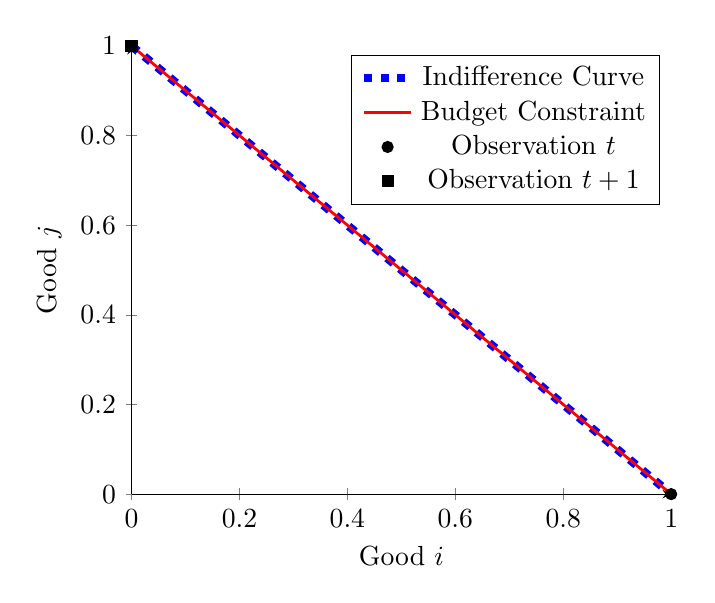
\begin{tikzpicture}
    \begin{axis}[
    axis lines = left,
    xlabel = Good $i$,
    ylabel = Good $j$
]
\addplot [
    domain=0:1, 
    samples=2, 
    color=blue,
    line width=3pt,
    dashed
]
{1-x};
\addlegendentry{Indifference Curve}
  \addplot [
    domain=0:1, 
    samples=2, 
    color=red,
    line width=1pt,
]
{1-x};
\addlegendentry{Budget Constraint}
\addplot [only marks] table {
1 0
};
\addlegendentry{Observation $t$}
\addplot [only marks, mark=square*] table {
0 1
};
\addlegendentry{Observation $t+1$}
    \end{axis}
\end{tikzpicture}
\caption{SARP vs. GARP} \label{fig:SARPvsGARP}
\end{figure}
\noindent
Note the straight line represent both the indifference curves \emph{and} budget constraints at time $t$ both times. Under these conditions, any choice along the budget constraint is rational. 

The following table and Venn Diagram summarizes the requirements for each of the axioms:

\renewcommand{\arraystretch}{1.5}
\begin{center}
\begin{tabular}{ c|c|c } 
Axiom & If $\ldots$ & Then $\ldots$ \\\hline
WARP&$X_i \mathbf{R_D} X_j$&$\neg(X_j \mathbf{R_D} X_i)$ \\
SARP&$X_i \mathbf{R} X_j$&$\neg(X_j \mathbf{R} X_i)$ \\
WGARP&$X_i  \mathbf{R_D} X_j$&$\neg(X_j \mathbf{R_{SD}} X_i)$ \\
GARP&$X_i \mathbf{R} X_j$&$\neg(X_j  \mathbf{R_{SD}} X_i)$
\end{tabular}
\end{center}
\renewcommand{\arraystretch}{1}


\begin{figure}[H]
\centering
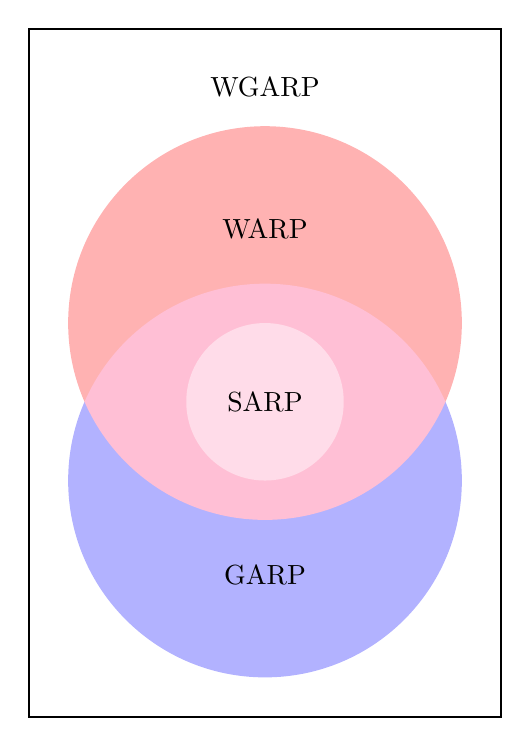
\begin{tikzpicture}
  \begin{scope}[blend group=soft light]
      \fill[red!30!white]   (90:2) circle (2.5);
    \fill[white!30!white] (90:1) circle (1);
    \fill[blue!30!white] (90:0) circle(2.5);
     \end{scope}
  \node at ( 90:3.2)    {WARP};
  \node at (90:1) {SARP};
  \node at (90:-1.2) {GARP};
  \node at (90:5) {WGARP};
    \draw[thick] ([shift={(-.5,-.5)}]current bounding box.south west) rectangle ([shift={(.5,.5)}]current bounding box.north east);
\end{tikzpicture}
\caption{Summary of Axioms} \label{fig:axioms_summary}
\end{figure}

The following graph further illustrates the relationships between each axiom:
\begin{figure}[H]
\centering
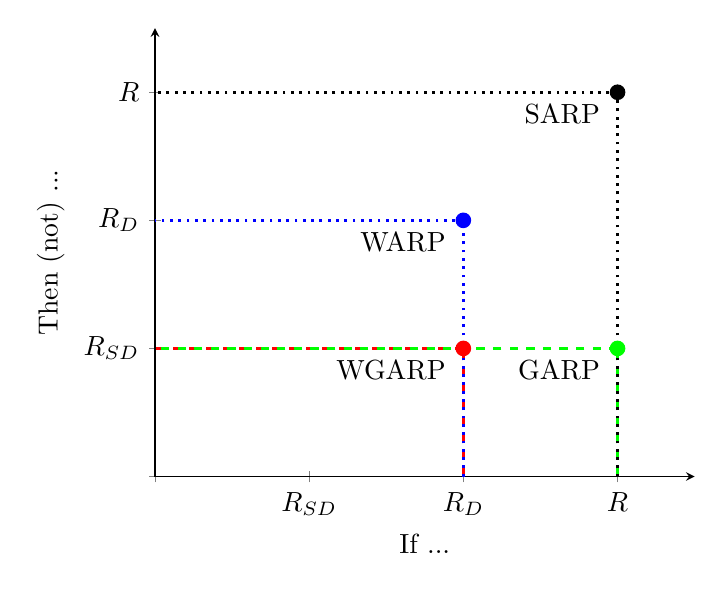
\begin{tikzpicture}
    \begin{axis}[
    axis lines = left,
    xlabel = If ...,
    ylabel = Then (not) ...,
    xmin=0,
    xmax=3.5,
    ymin=0,
    ymax=3.5,
    xtick = {0,1,2,3},
    ytick = {0,1,2,3},
    xticklabels = { ,$R_{SD}$, $R_D$, $R$},
    yticklabels = { ,$R_{SD}$, $R_D$, $R$},
]
\draw [dashed, color=red, line width=1pt] (2,0) -- (2,1);
\draw [dashed, color=red, line width=1pt] (2,1) -- (0,1);
\draw [dotted, color=blue, line width=1pt] (2,0) -- (2,2);
\draw [dotted, color=blue, line width=1pt] (2,2) -- (0,2);
\draw [dashed, color=green, line width=1pt] (3,0) -- (3,1);
\draw [dashed, color=green, line width=1pt] (3,1) -- (0,1);
\draw [dotted, color=black, line width=1pt] (3,0) -- (3,3);
\draw [dotted, color=black, line width=1pt] (3,3) -- (0,3);
\node[label={200:{WGARP}}, circle, fill, inner sep=2pt, color=red] at (axis cs:2,1) {};
\node[label={200:{WARP}}, circle, fill, inner sep=2pt, color=blue] at (axis cs:2,2) {};
\node[label={200:{GARP}}, circle, fill, inner sep=2pt, color=green] at (axis cs:3,1) {};
\node[label={200:{SARP}}, circle, fill, inner sep=2pt, color=black] at (axis cs:3,3) {};
    \end{axis}
\end{tikzpicture}
\caption{Axioms as Partial Orders} \label{fig:PartialOrder1}
\end{figure}

\section{Revealed Preferences as Directed Graphs}\label{sec:rev_pref_as_digraph}

This section will rigorously outline a graph theoretical approach to analyzing revealed preferences and introduce algorithms to test for each of the axioms. First, define two directed graphs, $G_d$ and $G_s$, that represent non-strict and strict relations between bundles, respectively. These conditions will yield:
$$G_d=\{\mathcal{X},E_d\}\textrm{ such that }E_d=\{(X_i,X_j)\ |\ X_i R_D X_j,\ i.e.\ P_iX_i\geq P_iX_j,\ i\not=j\}$$
$$G_s=\{\mathcal{X},E_s\}\textrm{ such that }E_s=\{(X_i,X_j)\ |\ X_i R_{SD} X_j,\ i.e.\ P_iX_i> P_iX_j,\ i\not=j\}$$
It is best to represent each graph with an adjacency matrix, where the $(i,j)^{th}$ element of the adjacency matrix is 1 if there's an edge from $X_i$ to $X_j$, 0 otherwise. The following paragraphs will discuss the construction of the adjacency matrices for $G_d$ and $G_s$, which will be denoted as $A_d$ and $A_s$, respectively.

Suppose an individual has choice data $\mathcal{X}=\{X_1,\ldots,X_k\}$ and $\mathcal{P}=\{P_1,\ldots,P_k\}$. One can then create the following $(k\times k)$ matrix from $\mathcal{X}$ and $\mathcal{P}$ (referred to as the expenditure matrix):
\[
Exp = 
 \begin{pmatrix}
  P_1X_1 & P_2X_1 & \cdots & P_kX_1 \\
  P_1X_2 & P_2X_2 & \cdots & P_kX_2 \\
  \vdots  & \vdots  & \ddots & \vdots  \\
  P_1X_k & P_2X_k & \cdots & P_kX_k
 \end{pmatrix}
\]
Note that the $(i,j)^{th}$ entry of this matrix represents the cost of bundle $i$ at the price of time $j$ (i.e. $P_jX_i$). Then consider the following:
\[
Exp_{diag} = 
 \begin{pmatrix}
  P_1X_1 & P_2X_2 & \cdots & P_kX_k \\
  P_1X_1 & P_2X_2 & \cdots & P_kX_k \\
  \vdots  & \vdots  & \ddots & \vdots  \\
  P_1X_1 & P_2X_2 & \cdots & P_kX_k
 \end{pmatrix}
\]
In $Exp_{diag}$, every element in column $j$ is same for all $j$ and represents the actual cost of bundle $j$ at the price vector it was bought at (price vector of time $j$). Then consider the following:
\[
\alpha = Exp-Exp_{diag} =
 \begin{pmatrix}
  0 & P_2X_1-P_2X_2 & \cdots & P_kX_1-P_kX_k \\
  P_1X_2-P_1X_1 & 0 & \cdots & P_kX_2-P_kX_k \\
  \vdots  & \vdots  & \ddots & \vdots  \\
  P_1X_k-P_1X_1 & P_2X_k-P_2X_2 & \cdots & 0
 \end{pmatrix}
\]
Define a function $f:\mathbb{R}\to\{0,1\}$ such that:
\[ 
f(x)=
    \begin{cases} 
      1 & x\leq0 \\
      0 & x>0
   \end{cases}
\]
Applying $f$ to all elements of $\alpha$ except its diagonals and take its transpose, one will obtain the adjacency matrix ($A_d$) for $G_d$:
\[
A_d =
 \begin{pmatrix}
  0 & f(\alpha_{1,2}) & \cdots & f(\alpha_{1,k}) \\
  f(\alpha_{2,1}) & 0 & \cdots & f(\alpha_{2,k}) \\
  \vdots  & \vdots  & \ddots & \vdots  \\
  f(\alpha_{k,1}) & f(\alpha_{k,2}) & \cdots & 0
 \end{pmatrix} ^T
\]
One can see that $A_d$ is in fact the adjacency matrix by considering the following:
\begin{itemize}
    \item $f(\alpha_{i,j})=1$ if and only if $\alpha_{i,j}\leq0$
    \item If $\alpha_{i,j}\leq0$, then $P_jX_i-P_jX_j\leq0$ and hence $P_jX_i\leq P_jX_j$
    \item Hence, by definition, $X_j R_D X_i$
    \item Thus $f(\alpha_{i,j})=1$ exactly when $X_j R_D X_i$
    \item However, a value of $1$ in $(i,j)$ position would indicate that a directed edge from vertex $i$ to vertex $j$, but since the edges need to indicate directly revealed preferences, one would want a value of $1$ at the $(j,i)$ positions. Hence, taking the transpose would result in $A_{d_{j,i}}=f(\alpha_{i,j})=1$ if and only if $X_j R_D X_i$, which is the desired adjacency matrix.
\end{itemize}
To construct $A_s$, consider the function $g:\mathbb{R}\to\{0,1\}$ such that:
\[ 
g(x)=
    \begin{cases} 
      1 & x<0 \\
      0 & x\geq0
   \end{cases}
\]
Similarly, applying $g$ to all elements of $\alpha$ except its diagonals and take its transpose would generate the adjacency matrix ($A_s$) for $G_s$:
\[
A_s =
 \begin{pmatrix}
  0 & g(\alpha_{1,2}) & \cdots & g(\alpha_{1,k}) \\
  g(\alpha_{2,1}) & 0 & \cdots & g(\alpha_{2,k}) \\
  \vdots  & \vdots  & \ddots & \vdots  \\
  g(\alpha_{k,1}) & g(\alpha_{k,2}) & \cdots & 0
 \end{pmatrix} ^T
\]
The intuition behind $A_s$ is similar to that of $A_d$ except the conditions of $g$ are set such that the relation between $X_i$ and $X_j$ need to be strict in order for $(i,j)$ to be 1.

Using the graph theoretical approach, one can reframe the relations on Definition \ref{defn:relations_1} as follows:
\begin{definition}\label{defn:relations_2} \leavevmode
\begin{enumerate}
  \circleditem For $X_i,X_j\in\mathcal{X}$, we say $X_i$ is \textbf{directly revealed preferred} to $X_j$ if there exists an edge from $X_i$ to $X_j$ on $G_d$, i.e. $(X_i,X_j)\in E_d$.
  \circleditem For $X_i,X_j\in\mathcal{X}$, we say $X_i$ is \textbf{strictly directly revealed preferred} to $X_j$ if there exists an edge from $X_i$ to $X_j$ on $G_s$, i.e. $(X_i,X_j)\in E_s$.
  \circleditem For $X_i,X_j\in\mathcal{X}$, we say $X_i$ is \textbf{revealed preferred} to $X_j$ if there's a walk (of any length) from $X_i$ to $X_j$ on $G_d$.
\end{enumerate}
\end{definition}
\noindent
Similarly, the axioms from Definition \ref{defn:axioms_1} is reframed as follows:

\begin{definition}\label{axioms_2} \leavevmode
\begin{enumerate}
  \circleditem A set of choice data satisfies the \textbf{Weak Axiom of Revealed Preferences (WARP)} if $\forall i,j\in\{1,\dots,k\}$ where $i\not=j$, if $(X_i,X_j)\in E_d$, then $(X_j, X_i)\not\in E_d$.
  \circleditem A set of choice data satisfies the \textbf{Strong Axiom of Revealed Preferences (SARP)} if $\forall X_i \in \mathcal{X}$, there exists no directed walk from $X_i$ back to itself.
  \circleditem A set of choice data satisfies the \textbf{Generalized Axiom of Revealed Preferences (GARP)} if $\forall i,j\in\{1,\dots,k\}$, if there exists a directed walk from $X_i$ to $X_j$ in $G_d$, then $(X_j,X_i)\not\in E_s$.
  \circleditem A set of choice data satisfies the \textbf{Weak Generalized Axiom of Revealed Preferences (WGARP)} if $\forall i,j\in\{1,\dots,k\}$ where $i\not=j$, if $(X_i,X_j)\in E_d$, then $(X_j, X_i)\not\in E_s$.
\end{enumerate}
\end{definition}
Suppose there exists a set of choice data for an individual given by $(\mathcal{X},\mathcal{P})$ where $|\mathcal{X}|=|\mathcal{P}|=k\in\mathbb{N}$. Let $A_d$ and $A_s$ be the adjacency matrices of $G_d$ and $G_s$ constructed from the data set, respectively. To test for each of the axioms, the paper proposes the following theorems.
\begin{restatable}{thm}{WARP}
\label{thm:WARP}
A set of choice data, $(\mathcal{X},\mathcal{P})$, satisfies WARP exactly when, $\forall i\in\{1,\ldots,k\}$, $(A_d)^2_{i,i}=0$.
\end{restatable}

WARP requirements are defined such that if $(\mathcal{X},\mathcal{P})$ passes WARP, then: $\forall i,j\in\{1,\dots,k\}$ where $i\not=j$, if $(X_i,X_j)\in E_d$, then $(X_j, X_i)\not\in E_d$. Note that this is true exactly when there \textit{isn't} a directed walk of length 2 from any vertex $i$ back to itself (vertex $i$). Hence we say $(\mathcal{X},\mathcal{P})$ passes WARP if and only if the main diagonal of matrix $(A_d)^2$ is a vector of 0, which is exactly the statement of Theorem \ref{thm:WARP}.

\begin{restatable}{thm}{SARP}
\label{thm:SARP}
A set of choice data, $(\mathcal{X},\mathcal{P})$, satisfies SARP exactly when, $\forall i\in\{1,\ldots,k\}$, $\big(\sum_{n=2}^k(A_d)^n\big)_{i,i}=0$.
\end{restatable}
Consider for $n\geq2$, $\big((A_d)^n\big)_{i,j}$ would represent the number of directed walks of length $n$ from $X_i$ to $X_j$. Let $B_d=\big(\sum_{n=2}^k(A_d)^n\big)$. Then $(B_d)_{i,j}>0$ if and only if there is a directed walk of at least length 2 from $X_i$ to $X_j$, as the cardinality of the vertex set is $k$ and adding above that index would simply be extra computation. Hence, $(B_d)$'s main diagonal is 0 if and only if no vertices has a directed walk back to itself, which is exactly the statement of Theorem \ref{thm:SARP}.

\begin{restatable}{thm}{WGARP}
\label{thm:WGARP}
A data set $(\mathcal{X}, \mathcal{P})$ passes WGARP if and only if, $\forall i\in\{1,\ldots,k\}$, $(A_d \times A_s)_{i,i}=0$ (i.e. the main diagonal of $A_d \times A_s$ is a vector of 0).
\end{restatable}

\begin{restatable}{thm}{GARP}
\label{thm:GARP}
A data set $(\mathcal{X},\mathcal{P})$ passes GARP if and only if, $\forall i\in\{1,\ldots,k\}$, $\big((\sum_{i=1}^{k-1}A_{d}^{i})\times A_s\big)_{i,i}=0$ (i.e. the main diagonal of $(\sum_{i=1}^{k-1}A_{d}^{i})\times A_s$ is a vector of 0).
\end{restatable}

The proofs of Theorem \ref{thm:WGARP} and Theorem \ref{thm:GARP} are in the Appendix. The basic idea behind these two algorithms are similar to that of Theorem \ref{thm:WARP} and Theorem \ref{thm:SARP}, except they are adjust to include the idea of strict revealed preferences that are a part of the axioms. This section will conclude with a few examples that exhibit the functionalities of the graph theoretical approach.

\begin{example}\label{ex1}

Consider the following data for a single consumer in 3 different time periods:
\begin{center}
\begin{tabular}{ cccccc } 
Choice Number & $p_{1}$ & $p_{2}$ & $x_{1}$ & $x_{2}$ \\
1&1&2&1&2 \\
2&2&1&2&1 \\
3&1&1&2&2
\end{tabular}
\end{center}
Then, $\forall n\in\{1,2,3\}$, calculate $P_{n}X_{n}$ and $\forall i,j\in\{1,2,3\}$ such that $i\not=j$, calculate $P_{j}X_{i}$. This will result in the following expenditure matrix:
\[
Exp = \begin{pmatrix}
5&4&3 \\
4&5&3 \\
6&6&4
\end{pmatrix}
\]
Using $Exp_{diag}$ as defined previously, calculate:
\[\alpha=Exp-Exp_{diag}=\begin{pmatrix}
0 &-1 &-1\\
-1&0&-1\\
1&1&0\\
\end{pmatrix}
\]
Applying $f$ to all non-diagonal elements of $\alpha$ and taking the inverse would result in the adjacency matrix, as follows:
\[
A_d=\begin{pmatrix}
0 & 1 & 0\\
1 & 0 &0 \\
1 & 1 & 0
\end{pmatrix}
\]
Since all the inequalities are strict in this case, we have $A_s=A_d$ and hence $G_s=G_d$. Consider the following graph, representing both $G_d$ and $G_s$:
\begin{figure}[H]
\centering
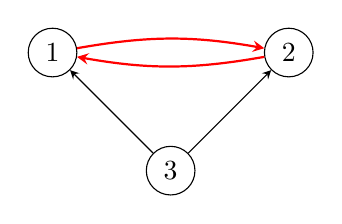
\begin{tikzpicture}[scale = 1.5]
\tikzset{
    vertex/.style={circle,draw,minimum size=1.5em},
    edge/.style={->,> = latex'}
}
  % vertices
\node[vertex] (1) at  (-1,0) {$1$};
\node[vertex] (2) at (1,0) {$2$};
\node[vertex] (3) at (0,-1) {$3$};
% edges
\path[->,>=stealth]
(1) edge[bend left=10,red,thick] (2)
(2) edge[bend left=10,red,thick] (1)
(3) edge (2)
(3) edge (1)
;
\end{tikzpicture}
\caption{Illustration of $G_d$ / $G_s$} \label{fig:example1_graph}
\end{figure}
Upon first glance, one can see that the revealed preferences between $X_1$ and $X_2$ indicates violations of all axioms. Since $G_d=G_s$, the individual's data set show that $(X_1,X_2)\in E_d = E_s$ and $(X_2,X_1)\in E_d=E_s$. This ``conflict'' is represented in the graph with the red arrows, creating a walk of 2 edges from $X_1$ back to itself (similarly with $X_2$). Theorem \ref{thm:WARP} states that, if the data set were to in fact fail WARP, there will be at least one non-zero element in the main diagonal of $(A_d)^2$. Using $A_d$ exhibited by the individual, one can see Theorem \ref{thm:WARP} holds:
\[
(A_d)^2=\begin{pmatrix}
0 & 1 & 0\\
1 & 0 &0 \\
1 & 1 & 0
\end{pmatrix}^2 = \begin{pmatrix}
1&0&0\\
0&1&0\\
1&1&0
\end{pmatrix}\]
Additionally, since $A_d=A_s$, $A_d\times A_s=A_d\times A_d=(A_d)^2$. Thus, the behavior exhibited by this individual fails WGARP as well.
\end{example}

\begin{example}\label{ex2}
The following example will explicit illustrate the differences between SARP and GARP. Consider the following expenditure matrix exhibited by a different consumer:
\[Exp = \begin{pmatrix}
236 & 232 & 176\\
236 & 222 & 186\\
250 & 222 & 176
\end{pmatrix}
\]
As before, one can obtain the matrix $\alpha$ as follows:
\[
\alpha = \begin{pmatrix}
0 & 10 & 0 \\
0 & 0 & 10 \\
14 & 0 & 0 \\
\end{pmatrix}
\]
In this case, $A_d\not=A_s$ as some bundles have non-strict revealed preferences to each other. Applying $f$ to obtain $A_d$ and $g$ to obtain $A_s$, one can obtain the following:

\begin{minipage}{0.5\linewidth}
\[A_d = \begin{pmatrix}
0 & 1 & 0\\
0 & 0 & 1 \\
1 & 0 & 0 \\
\end{pmatrix}
\]
\end{minipage}
\begin{minipage}{0.5\linewidth}
\[A_s = \begin{pmatrix}
0 & 0 & 0\\
0 & 0 & 0 \\
0 & 0 & 0 \\
\end{pmatrix}
\]
\end{minipage}
Since $G_d\not=G_s$, the data set can be represented with the following two graphs:
\begin{minipage}{0.5\linewidth}
\begin{figure}[H]
\centering
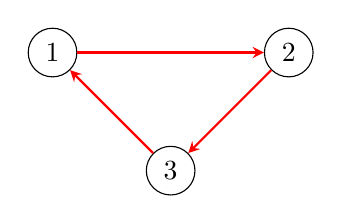
\begin{tikzpicture}[scale = 1.5]
\tikzset{
    vertex/.style={circle,draw,minimum size=1.5em},
    edge/.style={->,> = latex'}
}
  % vertices
\node[vertex] (1) at  (-1,0) {$1$};
\node[vertex] (2) at (1,0) {$2$};
\node[vertex] (3) at (0,-1) {$3$};
% edges
\path[->,>=stealth]
(1) edge[red,thick] (2)
(2) edge[red,thick](3)
(3) edge[red,thick](1)
;
\end{tikzpicture}
\caption{Illustration of $G_d$} \label{fig:example2_graph_Gd}
\end{figure}
\end{minipage}
\begin{minipage}{0.5\linewidth}
\begin{figure}[H]
\centering
\begin{tikzpicture}[scale = 1.5]
\tikzset{
    vertex/.style={circle,draw,minimum size=1.5em},
    edge/.style={->,> = latex'}
}
  % vertices
\node[vertex] (1) at  (-1,0) {$1$};
\node[vertex] (2) at (1,0) {$2$};
\node[vertex] (3) at (0,-1) {$3$};
% edges
\end{tikzpicture}
\caption{Illustration of $G_s$} \label{fig:example2_graph_Gd}
\end{figure}
\end{minipage}

As highlighted by the red edges, this data set fails SARP as there is a walk from all edges back to themselves on $G_d$. This can also be seen with the following computations:
\[\sum_{n=2}^3(A_d)^n=\begin{pmatrix}
0 & 1 & 0\\
0 & 0 & 1 \\
1 & 0 & 0 \\
\end{pmatrix}^2+
\begin{pmatrix}
0 & 1 & 0\\
0 & 0 & 1 \\
1 & 0 & 0 \\
\end{pmatrix}^3=
\begin{pmatrix}
1&0&1\\
1&1&0\\
0&1&1
\end{pmatrix}
\]
Note that $(\sum_{n=2}^3(A_d)^n)_{i,i}=1$ for all $i\in\{1,2,3\}$, thus the data set violates SARP by Theorem \ref{thm:SARP}. Further, it's clear that $\big( (\sum_{i=1}^{2}A_d^i)\times A_s \big)$ is the zero matrix as $A_s$ is the zero matrix, and hence the diagonal elements would all equal zero. This indicates that the data set passes GARP by Theorem \ref{thm:GARP}.
\end{example}

\section{Afriat's CCEI}

The purpose of this section is to develop a new algorithm, through a series of theorems, to compute Afriat's CCEI directly without a guess-and-check method\footnote{Note that this algorithm is more complex than existing guess-and-check methods. See \citet{CherchyeEtAl2014Goodness-of-Fit-Measures-for-Revealed-Preference-Tests:-Complexity-Results-and-Algorithms}}. First, the paper presents the precise definition of Afriat's CCEI with the following set of definitions. Let $\mathcal{X}$ and $\mathcal{P}$ be the set of quantity and price vectors, as defined previously and let $e\in[0.1]$, then:
\begin{definition}\label{defn:drp_e}
For $X_i,X_j\in\mathcal{X}$, we say $X_i$ is \textbf{e-directly revealed preferred} if $eP_iX_i\geq P_iX_j$. We will denote this as $X_i R_{D(e)}X_j$. Similarly, if $eP_iX_i > P_iX_j$, we say $X_i R_{SD(e)} X_j$.
\end{definition}

\begin{definition}\label{defn:rp_e}\leavevmode
We define $R_e$ be the transitive closure of $R_{D(e)}$. More specifically, for $X_i,X_j\in\mathcal{X}$, $X_iR_eX_j$ if there exists some sequence $\{X^m\}_{m=1}^M$ such that, $\forall m\in\{1,\ldots,M\}$, the following holds:
\begin{itemize}[topsep=0pt]
  \item $X^m\in\mathcal{X}$
  \item $X_i R_{D(e)} X^1$ i.e. $eP_iX_i\geq P_i X^1$
  \item $X^m R_{D(e)} X^{m+1}$ i.e. $e P^m X^m \geq P^m X^{m+1}$
  \item $X^M R_{D(e)}X_j$ i.e. $e P^M X^M\geq P^M X_j$
\end{itemize}  
\end{definition}

\begin{definition}\label{defn:GARPe}
Let $R_e$ be the transitive closure of $R_{D(e)}$. A set of choice data satisfies $GARP_e$ if for all bundles $X_i$ and $X_j$, if $X_i R_e X_j$, then $\neg (X_j R_{SD(e)} X_i)$. In other words, we say if $X_i R_e X_j$, then $eP_jX_j \leq P_iX_i$ (i.e. $eP_jX_j \not> P_iX_i$).
\end{definition}
Definition \ref{defn:drp_e} is simply the definition of direct revealed preference but parameterized by $e\in[0,1]$. Note that for $e=1$, this is precisely the definition of direct revealed preference (as stated in Definition \ref{defn:relations_1}). Definition \ref{defn:GARPe} is simply a ``relaxation'' of the standard GARP requirements. Additionally, one can see that by letting $e=0$, then any data set would pass GARP\textsubscript{e} since no bundle would even be revealed prefered to any other bundles! Thus, one can see that $\mathcal{E}_{(\mathcal{X},\mathcal{P})}=\{e\ |\ (\mathcal{X},\mathcal{P})\textrm{ passes GARP\textsubscript{e}}\textrm{ and } e\in[0,1]\}\not=\varnothing$ as $0\in\mathcal{E}_{(\mathcal{X},\mathcal{P})}$ for every possible dataset $(\mathcal{X},\mathcal{P})$.\footnote{In other words, for a given data set $(\mathcal{X},\mathcal{P})$, let $\mathcal{E}_{(\mathcal{X},\mathcal{P})}$ be the set of $e\in[0,1]$ such that $(\mathcal{X},\mathcal{P})$ passes GARP\textsubscript{e}. As shown, all data set $(\mathcal{X},\mathcal{P})$ would pass GARP\textsubscript{0}, thus we say for all $(\mathcal{X},\mathcal{P})$, $\mathcal{E}_{(\mathcal{X},\mathcal{P})}\not=\varnothing$.} We then obtain the following definition:

\begin{definition}\label{defn:Afriat_CCEI}
For data set $(\mathcal{X},\mathcal{P})$, \textbf{Afriat's CCEI} is the \emph{largest} value $e^*\in[0,1]$ such that $(\mathcal{X},\mathcal{P})$ passes $GARP_{e^*}$.
\end{definition}

Later examples will show that Afriat's CCEI often doesn't exist, as $\mathcal{E}_{(\mathcal{X},\mathcal{P})}$ may not be a closed set\footnote{Say $\mathcal{E}_{(\mathcal{X},\mathcal{P})}=[0,a)$ for some $a\in(0,1]$, then $\mathcal{E}_{(\mathcal{X},\mathcal{P})}$ does not have a largest element.} and thus does not have a ``largest'' value $e^*\in\mathcal{E}_{(\mathcal{X},\mathcal{P})}$. We then simply compute $e^*=\sup \mathcal{E}_{(\mathcal{X},\mathcal{P})}$ for data set $(\mathcal{X},\mathcal{P})$, which fails GARP\textsubscript{$e^*$} but for any $\epsilon>0$, passes GARP\textsubscript{$e^*-\epsilon$} (since $(e^*-\epsilon)\in \mathcal{E}_{(\mathcal{X},\mathcal{P})}$). Consider the following theorem regarding the nature of $\mathcal{E}_{(\mathcal{X},\mathcal{P})}$:

\begin{restatable}{thm}{AfriatConnected}\label{thm:Afriat_Connected}
Let $(\mathcal{X},\mathcal{P})$ be any data set (not contingent on passing / failing GARP) and define the set $\mathcal{E}_{(\mathcal{X},\mathcal{P})}=\{e\ |\ (\mathcal{X},\mathcal{P})\textrm{ passes GARP\textsubscript{e}}\textrm{ and } e\in[0,1]\}$ to be the collection of $e\in[0,1]$ such that $(\mathcal{X},\mathcal{P})$ passes GARP\textsubscript{e}. Then, $\mathcal{E}_{(\mathcal{X},\mathcal{P})}\subseteq[0,1]$ is a connected set.
\end{restatable}

Theorem \ref{thm:Afriat_Connected} ensures the existence of $e^*=\sup \mathcal{E}_{(\mathcal{X},\mathcal{P})}$ for all data sets $(\mathcal{X},\mathcal{P})$. The proof of the theorem is in the Appendix, althought its result can be easily seen by once one realizes that if $(\mathcal{X},\mathcal{P})$ passes GARP\textsubscript{$e'$} for some $e'\in[0,1]$, then it will also pass GARP\textsubscript{$e$} for all $e\in[0,e']$.

This section's main interest is to develop an algorithm to directly find Afriat's CCEI for a data set that does not pass the standard GARP requirements (since if $(\mathcal{X},\mathcal{P})$ passes GARP, its Afriat's CCEI would clearly be 1). Now define $G_d$ and $G_s$ as in Section \ref{sec:rev_pref_as_digraph} and suppose $(\mathcal{X},\mathcal{P})$ fails GARP, then there are $X_i,X_j\in\mathcal{X}$ where there's a directed walk from $X_i$ to $X_j$ in $G_d$ \emph{and} $(X_j,X_i)\in E_s$. The role of $e^*$ would be to ``relax'' those edges so that either the directed walk no longer exists or $(X_j,X_i)\not\in E_s$. More rigorously, one can create separate pairs of graphs for each $e\in[0,1]$: $G_{d(e)}=\{\mathcal{X},E_{d(e)}\}$ and $G_{s(e)}=\{\mathcal{X},E_{s(e)}\}$ where:
$$E_{d(e)}=\{(X_i,X_j)\ |\ X_iR_{D(e)}X_j\textrm{ i.e. } eP_iX_i\geq P_iX_j,\ i\not=j\}$$
$$E_{s(e)}=\{(X_i,X_j)\ |\ X_iR_{SD(e)}X_j\textrm{ i.e. } eP_iX_i> P_iX_j,\ i\not=j\}$$
To create an adjacency matrices for $G_{d(e)}$ and $G_{s(e)}$, one must adjust the expenditure matrix as follows:
\[
Exp_e=
\begin{pmatrix}
eP_1X_1 & P_2X_1 & \cdots & P_kX_1\\
P_1X_2 & eP_2X_2 & \cdots & P_kX_2\\
\vdots & \vdots & \ddots & \vdots \\
P_1X_k & P_2X_k & \cdots & eP_kX_k 
\end{pmatrix}
\]
and thus:
\[
Exp_{diag(e)}=
\begin{pmatrix}
eP_1X_1 & eP_2X_2 & \cdots & eP_kX_k \\
eP_1X_1 & eP_2X_2 & \cdots & eP_kX_k \\
\vdots & \vdots & \ddots & \vdots \\
eP_1X_1 & eP_2X_2 & \cdots & eP_kX_k 
\end{pmatrix}
\]
Let $\alpha_e=Exp_e-Exp_{diag(e)}$ and $i\not=j$ and one can see that $X_i R_{D(e)} X_j$ if and only if $(\alpha_e)_{j,i}=P_iX_j-eP_iX_i\leq0$ (as $P_iX_j-eP_iX_i\leq0 \iff eP_iX_i\geq P_iX_j$). Then, defining $f:\mathbb{R}\to\{0,1\}$ such that:
\[f(x)=\begin{cases}
1 & x\leq 0\\
0 & x>0
\end{cases}
\]
and $g:\mathbb{R}\to\{0,1\}$ such that:
\[g(x)=\begin{cases}
1 & x<0\\
0 & x\geq0
\end{cases}
\]
one can easily following the steps in Section \ref{sec:rev_pref_as_digraph} to construct $A_{d(e)}$ and $A_{s(e)}$ from $\alpha_e$ and $f, g$. Thus, given any $e\in[0,1]$, one can test whether $(\mathcal{X},\mathcal{P})$ passes GARP\textsubscript{e} with those adjacency matrices and the methods described in Section \ref{sec:rev_pref_as_digraph}.

In order to directly calculate Afriat's CCEI from a given data set $(\mathcal{X},\mathcal{P})$, one must reconstruct graphs $G_d$ and $G_s$ as weighted digraphs, which is a simply a directed graph with a weight function that assigns a real-valued weight to every edge. Let $\mathcal{X}=\{X_1,\ldots,X_k\}$ and $\mathcal{P}=\{P_1,\ldots,P_k\}$ and set up $G_d$ and $G_s$ as in Section \ref{sec:rev_pref_as_digraph}. Define functions $W_d:E_d\to\mathbb{R}_{\geq1}$ and and $W_s:E_s \to\mathbb{R}_{>1}$ so that $W_d(\varepsilon_d)$ is the weight of edge $\varepsilon_d\in E_d$ and $W_d(\varepsilon_s)$ is the weight of edge $\varepsilon_s\in E_s$. Let $\varepsilon_d =(X_i, X_j)\in E_d$ where $i\not=j$. Thus, by definition, $X_i R_D X_j$ and $P_iX_i\geq P_iX_j$. We define $W_d$ such that $W_d(\varepsilon_d)=\frac{P_iX_i}{P_iX_j}\geq 1$. Further, let $\varepsilon_s=(X_i, X_j)\in E_s$ for $i\not=j$. We then know that $X_i R_{SD} X_j$ and thus $P_iX_i>P_iX_j$. Then define $W_s(\varepsilon_s)=\frac{P_iX_i}{P_iX_j}>1$.

Now we create the weighted adjacency matrices (for $G_d$ and $G_s$) from our dataset. Let's consider our expenditure matrix, as given in the previous section:
\[
Exp = 
 \begin{pmatrix}
  P_1X_1 & P_2X_1 & \cdots & P_kX_1 \\
  P_1X_2 & P_2X_2 & \cdots & P_kX_2 \\
  \vdots  & \vdots  & \ddots & \vdots  \\
  P_1X_k & P_2X_k & \cdots & P_kX_k
 \end{pmatrix}
\]
Similarly, one could also retrieve a second matrix, $Exp_{diag}$, from it:
\[
Exp_{diag} = 
 \begin{pmatrix}
  P_1X_1 & P_2X_2 & \cdots & P_kX_k \\
  P_1X_1 & P_2X_2 & \cdots & P_kX_k \\
  \vdots  & \vdots  & \ddots & \vdots  \\
  P_1X_1 & P_2X_2 & \cdots & P_kX_k
 \end{pmatrix}
\]
We then create a matrix $Q$ such that:
\[
Q = Exp_{diag} \varoslash Exp
\]
where $\varoslash$ indicates division by element. Note that $Exp_{diag}$ and $Exp$ are both positive matrices with no zero element (under the weak assumption that the quantity vector has at least one non-zero element in it as prices are clearly always positive). More specifically, we have the following:
\[
Q = 
 \begin{pmatrix}
  1 & q_{1,2} & \cdots & q_{1,k} \\
  q_{2,1} & 1 & \cdots & q_{2,k} \\
  \vdots & \vdots & \ddots & \vdots \\
  q_{k,1} & q_{k,2} & \cdots & 1
 \end{pmatrix} =
 \begin{pmatrix}
 1 & \frac{P_2X_2}{P_2X_1} & \cdots & \frac{P_kX_k}{P_kX_1} \\[6pt]
 \frac{P_1X_1}{P_1X_2} & 1 & \cdots & \frac{P_kX_k}{P_kX_2} \\[6pt]
 \vdots & \vdots & \ddots & \vdots \\[6pt]
 \frac{P_1X_1}{P_1X_k} & \frac{P_2X_2}{P_2X_k} & \cdots & 1
 \end{pmatrix}
\]
Then we define two functions, $d:\mathbb{R}_{+}\to\mathbb{R}_{\geq1}\cup\{0\}$ and $s:\mathbb{R}_{+}\to\mathbb{R}_{>1}\cup\{0\}$, as follows:

\begin{minipage}{.5\linewidth}
\[ 
d(x)=
 \begin{cases} 
   x & x\geq1 \\
    0 & x<1
 \end{cases}
\]
\end{minipage}
\begin{minipage}{.5\linewidth}
\[
s(x)=
    \begin{cases} 
      x & x>1 \\
      0 & x\leq1
   \end{cases}
\]
\end{minipage}

Note that $d$ and $s$ are functions that will be applied to $Q$ for it to reflect the extent of either direct and strictly direct revealed preferences, with 0 being non-(strictly) directly revealed preferred. We then can define our adjacency matrices, $\Omega_d$ and $\Omega_s$ as follows (by applying $d,s$ to each element excpept the diagonals and setting the diagonals to 0, as there are no loops in our graph):
\[
\Omega_d =
  \begin{pmatrix}
  0 & d(q_{1,2}) & \cdots & d(q_{1,k}) \\
    d(q_{2,1}) & 0 & \cdots & d(q_{2,k}) \\
    \vdots & \vdots & \ddots & \vdots \\
    d(q_{k,1}) & d(q_{k,2}) & \cdots & 0
  \end{pmatrix}^T
\]

\[
\Omega_s =
  \begin{pmatrix}
  0 & s(q_{1,2}) & \cdots & s(q_{1,k}) \\
    s(q_{2,1}) & 0 & \cdots & s(q_{2,k}) \\
    \vdots & \vdots & \ddots & \vdots \\
    s(q_{k,1}) & s(q_{k,2}) & \cdots & 0
  \end{pmatrix} ^T
\]
Note that these are similar to $A_d$ and $A_s$ in Section \ref{sec:rev_pref_as_digraph} except that the matrix is no longer filled with binary elements but actually capture the extent of each preference. We shall briefly go over the reasoning behind why $\Omega_d$ is in fact the weighted adjacency matrix. The reader should follow similar logic to understand $\Omega_s$ as well. Let $i\not=j$ for simplicity and:
\begin{itemize}
  \item First note that $\Omega_{d_{i,j}}$ is in fact $d(q_{j,i})$.
  \item If $\Omega_{d_{i,j}}=d(q_{j,i})=0$, then $q_{j,i}<1$ and hence $\frac{P_iX_i}{P_iX_j}<1$ and thus $P_iX_i<P_iX_j$. We then get $\neg(X_i R_D X_j)$ so there's no edge between $X_i$ and $X_j$. Hence $\Omega_{d_{i,j}}=0$, as desired.
  \item If $\Omega_{d_{i,j}}=d(q_{j,i})\geq1$, then $q_{j,i}\geq1$ and hence $\frac{P_iX_i}{P_iX_j}\geq1$ and thus $P_iX_i\geq P_iX_j$. Thus we have an edge between $X_i$ and $X_j$ for $i\not=j$, as $X_iR_D X_j$, by definition. Then note that $d$ is in fact a bijective function (identity function) on the subset of the domain $[1,\infty)$ and that since $q_{j,i}\geq1$, by definition of $d$ we have $d(q_{j,i})=q_{j,i}$. Following definitions, we get $\Omega_{d_{i,j}}=d(q_{j,i})=q_{j,i}=\frac{P_iX_i}{P_iX_j}\geq1$, which is precisely the weight defined by $W_d$ earlier.
\end{itemize}

Before introducing a couple of theorems that pave way to the algorithm that allows for direct calculation of Afriat's CCEI, we provide a brief overview of the main idea behind the reasoning of algorithm. First, define a \emph{violating cycle} between $G_{d}$ and $G_{s}$ as a sequence $(X^k)_{k=1}^K$, where $X^k\in\mathcal{X}$ for all $k$ and there's a walk between $X^1$ and $X^K$ in $G_d$ and $(X^K,X^1)\in E_s$. Further, to avoid repetition and ensure finiteness of the number of total violating cycles, we also require $X^j\not=X^k$ for all $j,k\in\{1,\ldots,K\}$ where $j\not=k$ (that is, no edge is revisited during the walk).\footnote{This very last requirement is necessary as ilustrated by the following example. Consider $G_d=G_s$ where $\mathcal{X}=\{X_1,X_2\}$ and $E_s=E_d=\{(X_1,X_2),(X_2,X_1)\}$. Then, it's clear that $X_1 R X_2$ and $X_2 R_{SD} X_1$, therefore creating a violating cycle $(X^k)_{k=1}^2=(X_1,X_2)$. However, one can also argue that $(X^n)_{n=1}^4= (X_1,X_2,X_1,X_2)$ is also a violating cycle without the final requirement. However, the limited definition creates redundancies as the value of $e$ that removes the cycle $(X^k)_{k=1}^2$ would also remove $(X^n)_{n=1}^4$.} Let $\mathcal{V}$ denote the finite set of all violating cycles. Fixing $V\in\mathcal{V}$, we say that some $e\in[0,1]$ \emph{solves the violating cycle} if $V$ no longer exists on $G_{d(e)}$ and $G_{s(e)}$. More specifically, either the walk from $X^1$ to $X^K$ is no longer present in $G_{d(e)}$ or $(X^K,X^1)\not\in E_{s(e)}$. Consider the set
$$\mathcal{E}^V_{(\mathcal{X},\mathcal{P})} = \{e\in[0,1]\ |\ V\textrm{ is no longer present in } G_{d(e)}\textrm{ and } G_{s(e)} \}$$
It's clear that $0\in \mathcal{E}^V_{(\mathcal{X},\mathcal{P})}$ (the minimumal element) for all $V\in\mathcal{V}$ as $E_{s(0)}=\varnothing$. Further, $V\in\mathcal{V}$, $\mathcal{E}^V_{(\mathcal{X},\mathcal{P})}$ is a connected set and thus takes the form of either $[0,a)$ or $[0,a]$ for some $a\in(0,1]$. Naturally, if $e\in\mathcal{E}_{(\mathcal{X},\mathcal{P})}$, then it should solve all the violating cycles of $(\mathcal{X},\mathcal{P})$:
$$\mathcal{E}_{(\mathcal{X},\mathcal{P})} = \bigcap_{V\in\mathcal{V}}\mathcal{E}^V_{(\mathcal{X},\mathcal{P})} = \mathcal{E}^{V^*}_{(\mathcal{X},\mathcal{P})}$$
where $V^*\in\mathcal{V}$ is such that $\mathcal{E}^{V^*}_{(\mathcal{X},\mathcal{P})}\subseteq \mathcal{E}^V_{(\mathcal{X},\mathcal{P})}$ for all $V\in\mathcal{V}$. The above equality indicates that, to calculate the least upperbound of $\mathcal{E}_{(\mathcal{X},\mathcal{P})}$, one simply has to calculate the least upperbound of each $\mathcal{E}^V_{(\mathcal{X},\mathcal{P})}$ and take the minimum across $V\in\mathcal{V}$:
$$\sup \mathcal{E}_{(\mathcal{X},\mathcal{P})} = \min\left\{\sup \mathcal{E}^V_{(\mathcal{X},\mathcal{P})}\ |\ V\in\mathcal{V}\right\}$$
On the other hand, this is the same as analyzing all violating cycles $V\in\mathcal{V}$, finding the easiest edge to remove in each violating cycle (equivalent to finding least upperbound of each violating cycle), and determining the hardest cycle to remove based on their easiest edges (equivalent to taking the minimum across all violating cycles). 

To connect the above results to our approach with weighted digraphs, consider the following:
\begin{flalign*}\sup \mathcal{E}_{(\mathcal{X},\mathcal{P})} &= \left(\frac{1}{\min\left\{\sup \mathcal{E}^V_{(\mathcal{X},\mathcal{P})}\ |\ V\in\mathcal{V}\right\}}\right)^{-1} &\\ 
&= \left(\max\left\{\inf
\left(\mathcal{E}^V_{(\mathcal{X},\mathcal{P})}\right)^{-1}\ |\ V\in\mathcal{V}\right\}\right)^{-1}
\end{flalign*}
where every set $\left(\mathcal{E}^V_{(\mathcal{X},\mathcal{P})}\right)^{-1} = \left\{\frac{1}{e}\ |\ e\in \mathcal{E}^V_{(\mathcal{X},\mathcal{P})}\right\}$. Note then that, $\forall V\in\mathcal{V}$, we have $\sup \mathcal{E}^V_{(\mathcal{X},\mathcal{P})} = \frac{P_iX_j}{P_iX_i}$ for some $i,j\in\{1,\ldots,k\}$ where $i\not=j$ since either $\sup \mathcal{E}^V_{(\mathcal{X},\mathcal{P})}$ is supposed to remove an edge on $G_s$ or, $\forall \epsilon>0$, $\sup \mathcal{E}^V_{(\mathcal{X},\mathcal{P})} - \epsilon$ is supposed to remove a walk (by removing some edge along it) on $G_d$. Hence, $\forall V\in\mathcal{V}$, $\inf\left(\left(\mathcal{E}^V_{(\mathcal{X},\mathcal{P})}\right)^{-1}\right)$ is an element of $\Omega_d$ or $\Omega_s$ as it's of the form $\frac{P_iX_i}{P_iX_j}$. We can break down this definition even further. Note that every violating cycle $V\in\mathcal{V}$ two components: a walk between some $X_i$ to some $X_j$ in $G_d$ and $(X_j,X_i)\in E_s$. For all $V\in\mathcal{V}$, denote the walk component of $V$ as $\mathcal{L}_{V}$. As before, we define:
$$\mathcal{E}^{\mathcal{L}_{V}}_{(\mathcal{X},\mathcal{P})} = \{e\in[0,1]\ |\ \mathcal{L}_V\textrm{ is no longer present in }G_{d(e)}\textrm{ and }G_{s(e)}\}$$
Further, $\forall V\in\mathcal{V}$, define $e_V$ as \emph{the ratio of the edge }in $E_s$ associated with $V$. More specifically, fix $V$ and let $\mathcal{L}_V$ denote a walk from $X_i$ to $X_j$ on $G_d$, hence $(X_j,X_i)\in E_s$ and thus $e_V=\frac{P_jX_i}{P_jX_j}$ Then consider
\begin{flalign*}\sup \mathcal{E}_{(\mathcal{X},\mathcal{P})} &= \left(\max\left\{\inf\left(\mathcal{E}^V_{(\mathcal{X},\mathcal{P})}\right)^{-1}\ |\ V\in\mathcal{V}\right\}\right)^{-1} &\\
& = \left(\max\left\{\min\left\{\inf\left(\mathcal{E}^{\mathcal{L}_V}_{(\mathcal{X},\mathcal{P})}\right)^{-1},e_V^{-1}\right\}\ |\ V\in\mathcal{V}\right\}\right)^{-1}
\end{flalign*}
with each $\left(\mathcal{E}^{\mathcal{L}_V}_{(\mathcal{X},\mathcal{P})}\right)^{-1} = \left\{\frac{1}{e}\ |\ e\in \mathcal{E}^{\mathcal{L}_{V}}_{(\mathcal{X},\mathcal{P})} \right\}$. The last equality is apparent in that, fixing $V\in\mathcal{V}$, the greatest lower bound of the set $\left(\mathcal{E}^V_{(\mathcal{X},\mathcal{P})}\right)^{-1}$ would be the smaller value between the greatest lower bound of the walk associated with $V$ and $e_V^{-1}$, with the latter representing the ``edge component'' of the violating cycle $V$.

Now we begin to construct the algorithm for Afriat's CCEI.

First, define function $\lambda:\mathbb{R}^{m\times m} \times \mathbb{R}^{m\times m} \to \mathbb{R}^{m\times m}$ as follows:

Let $X,Y$ be $(m\times m)$ matrices and let $\lambda(X,Y)=Z$, then, $\forall i,j\in\{1,\ldots,m\}$:
$$Z_{i,j}=\max\{\min\{X_{i,1}, Y_{1,j}\}, \min\{X_{i,2}, Y_{2,j}\}, \ldots, \min\{X_{i,m}, Y_{m,j}\}\}$$
where $z_{i,j}$ is the $(i,j)^{th}$ element of $Z$. note that this is similar with matrix multiplication in that we consider the $i^{th}$ row of $X$ and $j^{th}$ column of $Y$, but instead of pairwise multiplication and overall summation (i.e. dot product), we take pairwise minimum and overall maximum.

We further define a function $\lambda_t:(\mathbb{R}^{m\times m})^t\to\mathbb{R}^{m\times m}$ such that for $Y_1,\ldots,Y_t\in \mathbb{R}^{m\times m}$, we have:
\[
  \lambda_t(Y_1,\ldots, Y_t) =
    \underbrace{\lambda(\cdots\lambda(\lambda(\lambda(}_\text{t-1 times}
    Y_1,Y_2),Y_3),Y_4),\ldots, Y_t)
\]
Consider the following set of theorems:
\begin{restatable}{thm}{CCEImain}
\label{thm:CCEI_main}
$\forall t\in \mathbb{N}_{\geq2}$,
\[
  \lambda_t(\underbrace{\Omega_d,\ldots,\Omega_d}_\text{t times})_{i,j}=
  \begin{cases}
  0 & \textrm{if } X_i, X_j\textrm{ are not connected by a walk of }t \textrm{ edges} \\
  & \textrm{on }G_d \\
  \rho_{i,j} & \textrm{such that }\rho_{i,j}\textrm{ is the weight of the strongest edge } \\
  &\textrm{among the weakest edges of all walks of } t \textrm{ edges} \\
  & \textrm{from }X_i\textrm{ to }X_j \textrm{ on } G_d
  \end{cases}
\]
We abbreviate $\lambda_t(\Omega_d,\ldots,\Omega_d)=\lambda^t(\Omega_d)$. Then, we formally write:
\[
  \lambda^t(\Omega_d)_{i,j}=
  \begin{cases}
  0 & \textrm{if } \nexists (X^v)_{v=1}^{t-1} \textrm{ such that } \forall v,\ X^v\in\mathcal{X}\textrm{ and } \\
  & (X^v,X^{v+1})\in E_d, (X_i,X^1)\in E_d \textrm{ and } \\
  & (X^{t-1},X_j)\in E_d\\ 
  \rho_{i,j} & \textrm{if }\exists (X^{uv})_{u,v=1}^{u=U,\ v=t-1}\ (\textrm{for some }U\geq1) \\
  & \textrm{such that }\forall u,\ \forall v,\ X^{uv}\in\mathcal{X} \textrm{ and } \\
  & (X^{uv},X^{u(v+1)})\in E_d\ (\textrm{if }t>2), (X_i, X^{u1})\in E_d \textrm{ and } \\
  & (X^{u(t-1)},X_j)\in E_d, \textrm{ then: } \\
  & \rho_{i,j}=\max\Big\{\min\big\{W_d\big((X_i,X^{u1})\big),W_d\big((X^{uv},X^{u(v+1)})\big), \\
  & W_d\big((X^{u(t-1)},X_j)\big)\ |\ v\in\{1,\ldots,t-2\}\big\}\ |\ u\in\{1,\ldots,U\}\Big\} \\
  &\textrm{if } t>2,\ \textrm{and }\\
  &\rho_{i,j}=\max\Big\{\min\big\{W_d\big((X_i,X^{u1})\big), W\big((X^{u1},X_j)\big)\big\}\ |\ u\in\\
  &\{1,\ldots,U\}\Big\} \textrm{ if } t=2\\
  \end{cases}
\]
Note that $\forall i,j$, $\rho_{i,j}\geq1$ since $W_d$ is the weight function as defined earlier. Further, intuitively, we say:
\[
  \lambda^t(\Omega_d)_{i,j}=
  \begin{cases}
  0 & \textrm{if bundles }X_i \textrm{ and }X_j\textrm{ are not connected by a} \\
  & \textrm{preference chain with } t { number of edges}\\
  \rho_{i,j} & \textrm{where }\rho_{i,j}\textrm{ is the largest ratio across the smallest ratios} \\
  & \textrm{in each preference chain that connects } X_i\textrm{ to } X_j \\ 
  & \textrm{with }t\textrm{ number of edges }
  \end{cases}
\]
\end{restatable}
The claim of Theorem \ref{thm:CCEI_main} can be better explained with the following illustration. Let $t=3$ and suppose that for $X_i,X_j\in\mathcal{X}$, the only walks that connect $X_i$ to $X_j$ with 3 edges are as follows:
\begin{figure}[H]
\centering
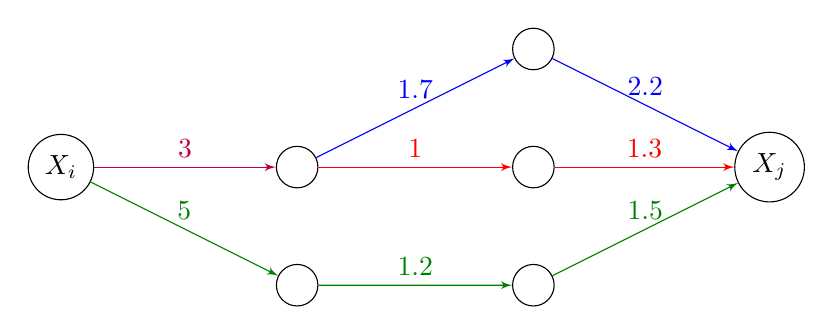
\begin{tikzpicture}[scale = 1.5]
\tikzset{
    vertex/.style={circle,draw,minimum size=1.5em},
    edge/.style={->,> = latex'}
}
  % vertices
\node[vertex] (1) at  (-3,0) {$X_i$};
\node[vertex] (3) at (1,1) {};
\node[vertex] (4) at (3,0) {$X_j$};
\node[vertex] (5) at (-1,0) {};
\node[vertex] (6) at (1,0) {};
\node[vertex] (7) at (-1,-1) {};
\node[vertex] (8) at (1,-1) {};
% edges
\draw[edge, color=blue] (3) -- (4) node[midway, above] {$2.2$};
\draw[edge, color=blue] (5) -- (3) node[midway, above] {$1.7$};
\draw[edge, color=purple] (1) -- (5) node[midway, above] {$3$};
\draw[edge, color=red] (5) -- (6) node[midway, above] {$1$};
\draw[edge, color=red] (6) -- (4) node[midway, above] {$1.3$};
\draw[edge, color=dark_green] (1) -- (7) node[midway, above] {$5$};
\draw[edge, color=dark_green] (7) -- (8) node[midway, above] {$1.2$};
\draw[edge, color=dark_green] (8) -- (4) node[midway, above] {$1.5$};
\end{tikzpicture}
\caption{Illustration of Theorem \ref{thm:CCEI_main}} \label{fig:example1_graph}
\end{figure}
One can see there are three distinct walks from $X_i$ to $X_j$, as colored with blue, red, and green (note that the edge from $X_i$ to the vertex just right of it, labelled with 3, belongs to both the blue and red walks). Then, Theorem \ref{thm:CCEI_main} claims that $\lambda^3(\Omega_d) = 1.7$ with $\Omega_d$ as the adjacency matrix for the weighted digraph that contains the illustrated paths. This can be seen as the smallest ratio of the blue preference chain is 1.7; the smallest ratio of the red preference chain is 1; and the smallest ratio of the green preference chain is 1.2, thus the maximum across those values is 1.7. The full proof of Theorem \ref{thm:CCEI_main} is quite lengthy and presented in the Appendix.

Now define a $k\times k$ matrix $\Lambda$ such that $\forall i,j\in\{1,\ldots,k\}$, we have that $\Lambda_{i,j}=\max\{\Omega_{d_{i,j}},\lambda^2(\Omega_d)_{i,j},\lambda^3(\Omega_d)_{i,j},\ldots,\lambda^{k-1}(\Omega_d)_{i,j}\}$. Hence $\Lambda$ is the element-wise maximization of matrices $\Omega_{d_{i,j}},\lambda^2(\Omega_d),\ldots,\lambda^{k-1}(\Omega_d)$. 

\begin{restatable}{cor}{CCEImainCor1}\label{thm:CCEI_mainCor1}
$\Lambda_{i,j}=\varrho_{i,j}\geq1$, $\forall i,j\{1,\ldots,k\}$ such that $i\not=j$, represents the weight of the strongest edge among the weakest edges of all walks, regardless the number of edges in the walks, from $X_i$ to $X_j$ on $G_d$.
\end{restatable}

\begin{restatable}{cor}{CCEImainCor2}\label{thm:CCEI_mainCor2}
If $\Lambda_{i,j}=0$, then $\nexists$ any walk from $X_i$ to $X_j$ on $G_d$.
\end{restatable}

\begin{restatable}{thm}{CCEIone}
\label{thm:CCEI_1}
$\forall i\in\{1,\ldots,k\}$, $\lambda(\Lambda,\Omega_s)_{i,i}=0$ if and only if the dataset $(\mathcal{X},\mathcal{P})$ has no GARP violations. 
\end{restatable}

\begin{restatable}{thm}{CCEItwo}
\label{thm:CCEI_2}
Let $\psi = \max\big\{\lambda(\Lambda,\Omega_s)_{i,i}\ |\ i\in\{1,\ldots,k\}\big\}$ and let $e^*=\frac{1}{\psi}$. The $e^*$ is the CCEI score related to the dataset $(\mathcal{X},\mathcal{P})$.
\end{restatable}

\section{Appendix}
\WGARP*

\begin{proof}
Recall that: If $(\mathcal{X},\mathcal{P})$ passes WGARP, then: $\forall i,j\in\{1,\dots,k\}$ where $i\not=j$, if $(X_i,X_j)\in E_d$, then $(X_j, X_i)\not\in E_s$. Which, when put in context of adjacency matrices, means that $\forall i,j\in\{1,\dots,k\}$ where $i\not=j$, if $(i,j)^{th}$ position of $A_d$ ($A_{d_{i,j}}$) is equal to one, then the $(j,i)^{th}$ position of $A_s$ ($A_{s_{i,j}}$) cannot be equal to 1. We then consider $A_d\times A_s$ and its main diagonal. 


$\forall i\in\{1,\ldots,k\}$, let $\delta_i$ be the vector of the $i^{th}$ row of $A_d$ and $\xi_i$ be the vector of the $i^{th}$ column of $A_s$. Then we have $(A_d\times A_s)_{i,i}=\delta_i\cdot\xi_i$. Note that $\delta_{i_i}=0$ and $\xi_{i_i}=0$ since originally $A_d$ and $A_s$ have all 0's across their main diagonals.


We then know that, $\forall i\in\{1,\ldots,k\}$, $(A_d\times A_s)_{i,i}=0$ (i.e. the main diagonal of $A_d\times A_s$ is a zero vector) if and only if $\delta_i\cdot\xi_i=0$. Further, $\delta_i\cdot\xi_i=0$ if and only if $\forall j \in\{1,\ldots,k\}$ such that $i\not=j$, $\delta_{i_j}\cdot \xi_{i_j}=0$ (since we know that $\delta_{i_i}=\xi_{i_i}=0$, they won't contributed to the overall sum, which is what we want anyways by the WGARP rules). We then know that $\delta_{i_j}\cdot \xi_{i_j}=0$ if and only if $\delta_{i_j}=0$ or $\xi_{i_j}=0$. Further, ``$\delta_{i_j}=0$ or $\xi_{i_j}=0$'' if and only if $\neg (\delta_{i_j}=\xi_{i_j}=1)$ (since all terms in $A_d$ and $A_s$ are either one or zero). Note that $\delta_{i_j}=A_{d_{i,j}}$ and $\xi_{i_j}=A_{s_{j,i}}$ (since $\xi_i$ is the vector of the $i^{th}$ \textit{column} of $A_s$). Hence, $\neg (\delta_{i_j}=\xi_{i_j}=1)$ if and only if $\neg (A_{d_{i,j}}=A_{s_{j,i}}=1)$, which happens if $A_{d_{i,j}}=1$, then $A_{s_{j,i}}=0\not=1$. Note that this is the exact definition of passing WGARP. Summarizing this, we have:
\begin{flalign*}
\forall i\in\{1,\ldots,k\}, (A_d\times A_s)_{i,i}=0 &\iff \delta_i\cdot\xi_i=0 &\\
&\iff \forall j \in\{1,\ldots,k\}\textrm{, }i\not=j,\ \delta_{i_j}\cdot \xi_{i_j}=0 &\\
&\iff \delta_{i_j}=0\textrm{ or }\xi_{i_j}=0 &\\
&\iff \neg (\delta_{i_j}=\xi_{i_j}=1) &\\
&\iff \neg (A_{d_{i,j}}=A_{s_{j,i}}=1) &\\
&\iff (A_{d_{i,j}}=1 \implies A_{s_{j,i}}=0\not=1)
\end{flalign*}

Hence, $\forall i, j\in\{1,\ldots,k\}$ such that $i\not=j$, $(A_d\times A_s)_{i,i}=0 \iff (A_{d_{i,j}}=1 \implies A_{s_{j,i}}=0\not=1)$. Note the first statement simply means the main diagonal of $A_d\times A_s$ is the zero vector and the second statement is the condition for passing WGARP. We then have ``passing WGARP'' $\iff$ ``main diagonal of $A_d\times A_s$ is a zero vector''. Thus our claim is proven (since $A\iff B$ is the same as $B\iff A$).
\end{proof}

\GARP*

Before we begin the proof, consider the following lemma:

\begin{lemma}
\label{lma:LemmaA}
Let $X_1, X_2, Y$ be $(m\times m)$ matrices such that:

\begin{minipage}{.5\linewidth}
\[
X_1 =
 \begin{pmatrix}
  x_{1,1} & x_{1,2} & \cdots & x_{1,m} \\
  x_{2,1} & x_{2,2} & \cdots & x_{2,m} \\
  \vdots  & \vdots  & \ddots & \vdots  \\
  x_{m,1} & x_{m,2} & \cdots & x_{m,m}
 \end{pmatrix}
\]
\end{minipage}
\begin{minipage}{.5\linewidth}
\[
X_2 =
 \begin{pmatrix}
  0 & x_{1,2} & \cdots & x_{1,m} \\
  x_{2,1} & 0 & \cdots & x_{2,m} \\
  \vdots  & \vdots  & \ddots & \vdots  \\
  x_{m,1} & x_{m,2} & \cdots & 0
 \end{pmatrix}
\]
\end{minipage}
and 

\[
Y =
 \begin{pmatrix}
  0 & y_{1,2} & \cdots & y_{1,m} \\
  y_{2,1} & 0 & \cdots & y_{2,m} \\
  \vdots  & \vdots  & \ddots & \vdots  \\
  y_{m,1} & y_{m,2} & \cdots & 0
 \end{pmatrix}
\]

Then the main diagonals of $X_1\times Y$ and $X_2\times Y$ are the same (denoted $diag(X_1\times Y)=diag(X_2\times Y)$).
\end{lemma}

\begin{proof}
Fix an arbitrary $i\in\{1,\ldots,m\}$. Then let $Z_1=X_1\times Y$ and $Z_2=X_2\times Y$. We want to show that $Z_{1_{i,i}}=Z_{2_{i,i}}$. Note that $Z_{1_{i,i}}=x_{i,1}y_{1,i}+x_{i,2}y_{2,i}+\ldots+x_{i,i}y_{i,i}+\ldots+x_{i,m}y_{m,i}$ and that $Z_{2_{i,i}}=x_{i,1}y_{1,i}+x_{i,2}y_{2,i}+\ldots+0y_{i,i}+\ldots+x_{i,m}y_{m,i}$. The only difference between those are that for the first equation, we have $x_{i,i}y_{i,i}$ as the $i^{th}$ term and the second equation, we have $0y_{i,i}$ as the $i^{th}$ term. However, since $y_{i,i}=0$, we have that $x_{i,i}y_{i,i}=0y_{i,i}=0$ and thus $Z_{1_{i,i}}=Z_{2_{i,i}}$.
\end{proof}

Now, consider the following proof for Theorem \ref{thm:GARP}:
\begin{proof}
The proof of this will look very similar to the proof of WGARP, except that the elements in $\sum_{i=1}^{k-1}A_{d}^{i}$ will no longer be binary $(\{0,1\})$. However, they are all $\geq0$. Let $\beta_d=\sum_{i=1}^{k-1}A_{d}^{i}$, then $\beta_{d_{i,j}}$ would be the number of directed walks between vertex $i$ and vertex $j$ of any length up to $k-1$. Note that we chose to sum up to $k-1$ since anything past that, we would definitely have a cycle and summing past that point is redundant.


We want to make sure that if there's a directed walk from vertex $i$ to vertex $j$ in $G_d$, there isn't a directed edge between vertex $j$ and vertex $i$ in $G_s$. Formally, this is just our definition for GARP: If $(\mathcal{X},\mathcal{P})$ passes GARP, then: $\forall i,j\in\{1,\dots,k\}$, if there exists a directed walk from $X_i$ to $X_j$ in $G_d$, then $(X_j,X_i)\not\in E_s$. This is similar to WGARP in the sense that we're simply replacing the directed edge in the ``if'' statement to a directed walk. Note then that we have $\beta_d=\sum_{i=1}^{k-1}A_{d}^{i}$, which captures the existence of any directed walks between any two verices. Hence if $\beta_{d_{i,j}}>0$, there exists at least 1 directed walk between vertex $i$ and vertex $j$ on graph $G_d$. We can then use our proof for WGARP and \textit{Lemma A} to construct the rest of this proof.


In our proof of WGARP, we see that $\forall i, j\in\{1,\ldots,k\}$ such that $i\not=j$, $(A_d\times A_s)_{i,i}=0 \iff (A_{d_{i,j}}=1 \implies A_{s_{j,i}}=0\not=1)$. There are two changes we need to make to this statement to fit our GARP claim. 

First, we see that we're no longer working with $A_d$ but working with $\beta_d$, which represents directed walks instead of edges. $\beta_d$ is also no longer filled with binary elements $\in\{0,1\}$. We can tweak our statement to fit these conditions by stating: $\forall i, j\in\{1,\ldots,k\}$ such that $i\not=j$, $(\beta_d\times A_s)_{i,i}=0 \iff (\beta_{d_{i,j}}>0 \implies A_{s_{j,i}}=0)$. Now, $\beta_{d_{i,j}}>0$ simply means there exists at least one path from $i,j$ regardless of length, which is what we want.

Second, when we constructed our proof of WGARP, we noted that ``since we know that $\delta_{i_i}=\xi_{i_i}=0$ (i.e. $A_{d_{i,i}}=0$ and $A_{s_{i,i}}=0$), they won't contributed to the overall sum, which is what we want anyways by the WGARP rules''. However, this no longer holds as we could have $\beta_{d_{i,i}}\not=0$ for some $i$ if there's any directed cycles in $G_d$ (but we don't care about those in GARP, per the definition of the axiom). But we do still have $A_{s_{i,i}}=0$ for all $i$ and thus, by \textit{Lemma A}, we don't need to ``clear-out'' the diagonals of $\beta_d$ before multiplying. Hence, our statement above still holds. 

Thus, we have: $\forall i, j\in\{1,\ldots,k\}$ such that $i\not=j$, $(\beta_d\times A_s)_{i,i}=0 \iff (\beta_{d_{i,j}}>0 \implies A_{s_{j,i}}=0)$. The first statement simply means the main diagonal of $(\beta_d=\sum_{i=1}^{k-1}A_{d}^{i}\times A_s)$ is a zero vector and the second statement is the condition for passing GARP, hence our proof is complete (since $A\iff B$ is the same as $B\iff A$).
\end{proof}

\AfriatConnected*
Before we prove Theorem \ref{thm:Afriat_Connected}, consider the following lemma:

\begin{lemma}\label{Lemma:Connectedness}
Let $e'\in[0,1]$ and $(\mathcal{X},\mathcal{P})$ be a data set that passes GARP\textsubscript{$e'$}. Then, for all $e\in[0,e']$, $(\mathcal{X},\mathcal{P})$ passes GARP\textsubscript{$e$}.
\end{lemma}
\begin{proof}
Suppose $(\mathcal{X},\mathcal{P})$ passes GARP\textsubscript{$e'$} for some $e'\in[0,1]$. Then, using the graph theoretical approach, $\forall X_i,X_j\in\mathcal{X}$, if there exists a directed walk from $X_i$ to $X_j$ on $G_{d(e')}$, then $(X_j,X_i)\not\in E_{s(e')}$. Note that any directed walk in $G_{d(e')}$ is simply a sequence of edges in $E_{d(e')}$. Now, let $e\in[0,e']$ and consider $G_{d(e)}$ and $G_{s(e)}$. The corresponding edge sets would then be $E_{d(e)}$ and $E_{s(e)}$. Note that for all $X_i,X_j\in\mathcal{X}$, $(X_i,X_j)\in  E_{d(e')}$ if and only if $e'P_iX_i\geq P_iX_j$ and, similarly,  $(X_i,X_j)\in  E_{s(e')}$ if and only if $e'P_iX_i>P_iX_j$. Since $e\leq e'$, we now have the following important conclusion: $$E_{d(e)}\subseteq E_{d(e')}\textrm{ and }E_{s(e)}\subseteq E_{s(e')}$$ Hence, by lowering $e$ from $e'$, no edges would be added upon $G_{d(e')}$ and $G_{s(e')}$. Therefore, no new directed walks would be created in $G_{d(e')}$ and no new edges would be created in $G_{s(e')}$. From this conclusion, we now know that $\forall X_i,X_j\in\mathcal{X}$, if there exists a directed walk from $X_i$ to $X_j$ on $G_{d(e)}$, then $(X_j,X_i)\not\in E_{s(e)}$. By definition, $(\mathcal{X},\mathcal{P})$ passes GARP\textsubscript{$e$}.
\end{proof}

Now we begin the proof of Theorem \ref{thm:Afriat_Connected}.
\begin{proof}
Let $(\mathcal{X},\mathcal{P})$ be a data set and define $\mathcal{E}_{(\mathcal{X},\mathcal{P})}=\{e\ |\ (\mathcal{X},\mathcal{P})\textrm{ passes GARP\textsubscript{e}}\\ \textrm{and } e\in[0,1]\}$. Suppose towards a contradiction that $\mathcal{E}_{(\mathcal{X},\mathcal{P})}$ is not connected and that two disjoint open sets, $U_1$ and $U_2$, form a separation of $\mathcal{E}_{(\mathcal{X},\mathcal{P})}$. That is, by definition, $\exists U_1,U_2$ (open sets) such that $U_1\cap U_2=\varnothing$, $\mathcal{E}_{(\mathcal{X},\mathcal{P})}\cap U_1\not=\varnothing$, $\mathcal{E}_{(\mathcal{X},\mathcal{P})}\cap U_2\not=\varnothing$, and $\mathcal{E}_{(\mathcal{X},\mathcal{P})}=(\mathcal{E}_{(\mathcal{X},\mathcal{P})}\cap U_1)\cup (\mathcal{E}_{(\mathcal{X},\mathcal{P})}\cap U_2)$. Without loss of generality, assume that for all $u_2\in U_2, u_1\in U_1$, $u_2>u_1$ (which is possible as $U_1\cap U_2=\varnothing$). Further, since $\mathcal{E}_{(\mathcal{X},\mathcal{P})}\subseteq [0,1]$ and $\mathcal{E}_{(\mathcal{X},\mathcal{P})}\cap U_i\not=\varnothing$ for $i=1,2$, we know $\exists x\in[0,1]$ such that $u_1<x<u_2$ for all $u_1,u_2$ (otherwise the separation between $U_1$ and $U_2$ would occur outside $[0,1]$ and for some $i=1,2$, we would get $\mathcal{E}_{(\mathcal{X},\mathcal{P})}\cap U_i=\varnothing$). Thus, $x\not\in U_1$ and $x\not\in U_2$ and, as $\mathcal{E}_{(\mathcal{X},\mathcal{P})}=(\mathcal{E}_{(\mathcal{X},\mathcal{P})}\cap U_1)\cup (\mathcal{E}_{(\mathcal{X},\mathcal{P})}\cap U_2)$, we would get $x\not\in\mathcal{E}_{(\mathcal{X},\mathcal{P})}$. However, as $\mathcal{E}_{(\mathcal{X},\mathcal{P})}\cap U_2\not=\varnothing$, $\exists u_2'\in \mathcal{E}_{(\mathcal{X},\mathcal{P})}\cap U_2$ such that $u_2'\in  \mathcal{E}_{(\mathcal{X},\mathcal{P})}$ and $u_2'>x$ (since $u_2'\in U_2$ and, $\forall u_2\in U_2$, $u_2>x$). By Lemma \ref{Lemma:Connectedness}, $x\in\mathcal{E}_{(\mathcal{X},\mathcal{P})}$, which is a contradiction.
\end{proof}



\CCEImain*

Before we begin the proof of Theorem \ref{thm:CCEI_main}, consider the following lemma.

\begin{lemma}\label{lemma:minmax_dist}
For all $\alpha^j_i\in\mathbb{R}$ and $\beta\in\mathbb{R}$, the following equality holds:
\[
\min
\left\{
  \begin{aligned}
    \max\left\{
      \begin{aligned}
        \min\{\alpha_1^1,&\ldots,\alpha_1^J\}, \\
        &\vdots \\
        \min\{\alpha_I^1,&\ldots,\alpha_I^J\}
      \end{aligned}
    \right\}
  \end{aligned}
  , \beta
\right\}
=
\max\left\{
  \begin{aligned}
    \min\{\alpha_1^1,&\ldots,\alpha_1^J,\beta\}, \\
    &\vdots \\
    \min\{\alpha_I^1,&\ldots,\alpha_I^J,\beta\} \\
  \end{aligned}
\right\}
\]
\end{lemma}

\begin{proof}
Considering the LHS, we have that:
\[
LHS=
\begin{cases}
\beta & \textrm{if } \beta\leq
\max\left\{
      \begin{aligned}
        \min\{\alpha_1^1,&\ldots,\alpha_1^J\}, \\
        &\vdots \\
        \min\{\alpha_I^1,&\ldots,\alpha_I^J\}
      \end{aligned}
    \right\} \\
    \\
\alpha_x^y\not=\beta &\textrm {if } \alpha_x^y\leq\alpha_x^1,\ldots,\alpha_x^J \textrm{ and} \\
& \alpha_x^y\geq \min\{\alpha_1^1,\ldots,\alpha_1^J\},\ldots,\min\{\alpha_I^1,\ldots,\alpha_I^J\} \textrm { and}\\
& \alpha_x^y\leq \beta
\end{cases}
\]
We can further write this as:
\[
LHS=
\begin{cases}
\beta & \textrm{if }\exists\ i_1\in\{1,\ldots,I\} \textrm{ such that }\forall j\in\{1,\ldots,J\}, \beta\leq\alpha_{i_1}^j \\
\alpha_x^y\not=\beta & \textrm{if } \alpha_x^y\leq\alpha_x^j,\ \forall j\in\{1,\ldots,J\} \textrm{ and} \\
& \forall i\in\{1,\ldots,I\},\ \exists\ j\in\{1,\ldots,J\} \textrm{ such that } \alpha_x^y\geq\alpha_i^j \textrm{ and } \\
& \alpha_x^y\leq \beta
\end{cases}
\]
Now consider the RHS, we have:
\[
RHS = 
\begin{cases}
\beta & \textrm{if }\exists\ i_1\in\{1,\ldots,I\} \textrm{ such that }\forall j\in\{1,\ldots,J\}, \beta\leq\alpha_{i_1}^j\ (*) \\
& \textrm{i.e. } \beta\geq\alpha_{i_1}^1,\ldots,\alpha_{i_1}^J\\
\alpha_x^y\not=\beta &\textrm{if }\alpha_x^y\leq\beta\ (***) \textrm{ and}\\
& \alpha_x^y\leq\alpha_x^1,\ldots,\alpha_x^J \textrm{ and}\\
& \alpha_x^y\geq \min\{\alpha_1^1,\ldots,\alpha_1^J,\beta\},\ldots,\min\{\alpha_I^1,\ldots,\alpha_I^J,\beta\}\ (**)
\end{cases}
\]
Looking at $(*)$, the condition ``$\exists\ i_1\in\{1,\ldots,I\} \textrm{ such that }\forall j\in\{1,\ldots,J\}, \beta\leq\alpha_{i_1}^j$'' suffices because under such condition, $RHS=\max\{\beta, \alpha_{i_2}\ |\ i_2\in I_2\}$ where $I_2\subseteq I$ is the set of $i\in I$ such that $\forall i_2\in I_2$, $\min\{\alpha_{i_2}^1,\ldots,\alpha_{i_2}^J,\beta\}=\alpha_{i_2}\not=\beta$. By the definition of the minimum, we then have: $\alpha_{i_2}\leq\beta$ and hence, $RHS=\max\{\beta, \alpha_{i_2}\leq\beta\ |\ i_2\in I_2\}=\beta$, as desired.

We then look at $(**)$: $\alpha_x^y\geq \min\{\alpha_1^1,\ldots,\alpha_1^J,\beta\},\ldots,\min\{\alpha_I^1,\ldots,\alpha_I^J,\beta\}$. We can rewrite this condition as: $\alpha_x^y\geq \min\big\{\min\{\alpha_1^1,\ldots,\alpha_1^J\},\beta\big\},\ldots,\min\big\{\min\{\alpha_I^1,\\\ldots,\alpha_I^J\},\beta\big\}$. We then claim that, given the conditions of $(***)$, it suffices to write: $\alpha_x^y\geq \min\big\{\min\{\alpha_1^1,\ldots,\alpha_1^J\}\big\},\ldots,\min\big\{\min\{\alpha_I^1,\ldots,\alpha_I^J\}\big\}$ and hence $\alpha_x^y\geq \min\{\alpha_1^1,\ldots,\alpha_1^J\},\ldots,\min\{\alpha_I^1,\ldots,\alpha_I^J\}$. The following is a brief proof:

Suppose towards a contradiction that the condition written above does not suffice and the entire condition, $\alpha_x^y\geq \min\big\{\min\{\alpha_1^1,\ldots,\alpha_1^J\},\beta\big\},\ldots,\min\big\{\min\{\alpha_I^1,\\\ldots,\alpha_I^J\},\beta\big\}$, is required. Then, we know that $\exists i\in\{1,\ldots,I\}$ such that $\min\big\{\min\{\alpha_i^1,\ldots,\alpha_i^J\},\beta\big\}=\beta$. We then have that $\alpha_x^y\geq\beta$, but by $(***)$, we also have $\alpha_x^y\leq\beta$, hence we have $\alpha_x^y=\beta$, which is a direct contradiction to the initial condition of $\alpha_x^y\not=\beta$. Hence, we know that it suffices to write $\alpha_x^y\geq \min\{\alpha_1^1,\ldots,\alpha_1^J,\beta\},\ldots,\min\{\alpha_I^1,\ldots,\alpha_I^J,\beta\}$ as $\alpha_x^y\geq \min\{\alpha_1^1,\ldots,\alpha_1^J\},\ldots,\min\{\\ \alpha_I^1,\ldots,\alpha_I^J\}$, given $(***)$.

Putting this all together, we have the following for the $RHS$:
\[
RHS=
\begin{cases}
\beta & \textrm{if }\exists\ i_1\in\{1,\ldots,I\} \textrm{ such that }\forall j\in\{1,\ldots,J\}, \beta\leq\alpha_{i_1}^j \\
\alpha_x^y\not=\beta & \textrm{if } \alpha\leq\beta \textrm{ and}\\
& \forall i\in\{1,\ldots,I\}, \exists\ j\in\{1,\ldots,J\}, \textrm{ such that } \alpha_x^y\geq\alpha_i^j \textrm{, and}\\
& \alpha_x^y\leq\alpha_x^j,\ \forall j\in\{1,\ldots,J\}
\end{cases}
\]

Note then that $LHS=RHS$ and hence our lemma is proven.
\end{proof}

Now we shall prove Theorem \ref{thm:CCEI_main}.

\begin{proof}
We approach this with proof by induction.

\textbf{Base Case:} Let $t=2$, we then have $\lambda_2(\Omega_d,\Omega_d)=\lambda(\Omega_d,\Omega_d)$. Set arbitrary $i,j\in\{1,\ldots,k\}$ and consider:
\begin{flalign*}
\lambda(\Omega_d,\Omega_d)_{i,j} &=\max\big\{\min\{\Omega^d_{i,1},\Omega^d_{1,j}\},\ldots,\min\{\Omega^d_{i,k},\Omega^d_{k,j}\}\big\} &\\
& =\max\big\{\min\{\Omega^d_{i,f},\Omega^d_{f,j}\}\ |\ f\in\{1,\ldots,k\}\big\}
\end{flalign*}
We then consider two cases:

\circled{1} If $\forall f\in\{1,\ldots,k\}$, $\Omega^d_{i,f}=0$ or $\Omega^d_{f,j}=0$, then $\lambda(\Omega_d,\Omega_d)_{i,j}=0$ as $\forall i,j\in\{1,\ldots,k\}$, $\Omega^d_{i,j}\in\{0\}\cup\mathbb{R}_{\geq1}$. Thus, if $\forall f\in\{1,\ldots,k\}$, $\Omega^d_{i,f}=0$ or $\Omega^d_{f,j}=0$, then $\lambda(\Omega_d,\Omega_d)_{i,j}=\max\{0,\ldots,0\}=0$.

\circled{2} Suppose $\exists F\subseteq\{1,\ldots,k\}$ (where $F\not=\varnothing$) such that $\forall f\in F$, $\Omega^d_{i,f}\geq1$ and $\Omega^d_{f,j}\geq1$. We then have $\lambda(\Omega_d,\Omega_d)_{i,j}=\max\big\{\min\{\Omega^d_{i,f},\Omega^d_{f,j}\}, 0\ |\ f\in F\big\}=\max\big\{\min\{\Omega^d_{i,f},\Omega^d_{f,j}\}\ |\ f\in F\big\}$.

Considering \circled{1} and \circled{2}, we have precisely the definition in our claim:

For \circled{1}, if $\nexists f$ such that $\Omega^d_{i,f}\geq1$ and $\Omega^d_{f,j}\geq1$, then we know $(X_i,X_f)\not\in E_d$ or $(X_f, X_j)\not\in E_d$ for all $f\in\{1,\ldots,k\}$. Hence, $\nexists (X^v)_{v=1}^1=X^v$ such that $X^v\in \mathcal{X}$ and $(X_i,X^v)\in E_d$ and $(X^v,X_j)\in E_d$, which is precisely our condition in the first case of the formalized version of our claim.

For \circled{2}, we have that $\lambda(\Omega_d,\Omega_d)_{i,j}=\max\big\{\min\{\Omega^d_{i,f},\Omega^d_{f,j}\}\ |\ f\in F\big\}$, where $\varnothing\not=F\subseteq\{1,\ldots,k\}$ such that $\forall f\in F$, $\Omega^d_{i,f}\geq1$ and $\Omega^d_{f,j}\geq1$. We then know that, $\forall f\in F$, $(X_i,X_f)\in E_d$ and $(X_f,X_j)\in E_d$. Then, we know that $\exists(X^{uv})_{u,v=1}^{u=U,\ v=1}=(X^{u1})_{u=1}^{U}$ (for $U=|F|$) such that $\forall u$, $X^{u1}\in\mathcal{X}$ and $(X_i,X^{u1})\in E_d$ and $(X^{u1},X_j)\in E_d$. We then have:
\begin{flalign*}
\lambda(\Omega_d,\Omega_d)_{i,j} &= \max\big\{\min\{\Omega^d_{i,f},\Omega^d_{f,j}\}\ |\ f\in F\big\} &\\
& = \max\big\{\min\{W_d\big((X_i, X_f)\big), W_d\big((X_f,X_j)\big)\}\ |\ f\in F\big\} &\\
& = \max\big\{\min\{W_d\big((X_i, X^{u1})\big), W_d\big((X^{u1},X_j)\big)\}\ |\ u\in\{1,\ldots,U\}\big\} &\\
& \textrm{ by construction of } F \textrm{ and }(X^{u1})_{u=1}^{U}
\end{flalign*}
Which is precisely our value in the second case of the formalized version of our claim. Combining those, our base case is complete.

\textbf{Inductive Case:} Let $t=n>2$, we then have: 
\[
\lambda_n(\underbrace{\Omega_d,\ldots,\Omega_d}_\text{n times})=\underbrace{\lambda(\cdots\lambda(\lambda(\lambda(}_\text{n-1 times}
    \Omega_d,\Omega_d),\Omega_d),\Omega_d,\ldots, \Omega_d)
\]

For the ease of notation, we will denote the matrix $\lambda_n(\Omega_d,\ldots,\Omega_d)=\lambda^n(\Omega_d)$. We then assume the following:
\[
\lambda^n(\Omega_d)_{i,j}=
\begin{cases}
0 & \textrm{if } \nexists (X^v)_{v=1}^{n-1} \textrm{ such that } \forall v,\ X^v\in\mathcal{X}\textrm{ and } \\
  & (X^v,X^{v+1})\in E_d, (X_i,X^1)\in E_d \textrm{ and } \\
  & (X^{n-1},X_j)\in E_d\\ 
\rho_{i,j} & \textrm{if }\exists (X^{uv})_{u,v=1}^{u=U,\ v=n-1}\ (\textrm{for some }U\geq1) \\
  & \textrm{such that }\forall u,\ \forall v,\ X^{uv}\in\mathcal{X} \textrm{ and } \\
  & (X^{uv},X^{u(v+1)})\in E_d, (X_i, X^{u1})\in E_d \textrm{ and } \\
  & (X^{u(n-1)},X_j)\in E_d, \textrm{ then: } \\
  & \rho_{i,j}=\max\Big\{\min\big\{W_d\big((X_i,X^{u1})\big),W_d\big((X^{uv},X^{u(v+1)})\big), \\
  & W_d\big((X^{u(n-1)},X_j)\big)\ |\ v\in\{1,\ldots,n-2\}\big\}\ |\ u\in\{1,\ldots,U\}\Big\}
\end{cases}
\]
Now let $t=n+1$, we then have:
\begin{flalign*}
\lambda_{n+1}(\underbrace{\Omega_d,\ldots,\Omega_d}_\text{n+1 times}) &=\underbrace{\lambda\bigl(\cdots\lambda(\lambda(\lambda(}_\text{n times}
    \Omega_d,\Omega_d),\Omega_d),\Omega_d,\ldots, \Omega_d \bigr) &\\
& =\lambda\bigl(\underbrace{\lambda(\cdots\lambda(\lambda(\lambda(}_\text{n-1 times}
    \Omega_d,\Omega_d),\Omega_d),\Omega_d,\ldots, \Omega_d),\Omega_d\bigr) &\\
& =\lambda\bigl(\lambda_n(\underbrace{\Omega_d,\ldots,\Omega_d}_\text{n times}),\Omega_d\bigr) &\\
& =\lambda\bigl(\lambda^n(\Omega_d),\Omega_d\bigr)
\end{flalign*}

Similarly, we denote $\lambda_{n+1}(\Omega_d,\ldots,\Omega_d)=\lambda^{n+1}(\Omega_d)$. We then have:
\begin{flalign*}
\lambda^{n+1}(\Omega_d)_{i,j} &=\lambda\bigl(\lambda^n(\Omega_d),\Omega_d\bigr)_{i,j} &\\
& =\max\bigl\{\min\{\lambda^n(\Omega_d)_{i,l},\Omega^d_{l,j}\}\ |\ l\in\{1,\ldots,k\}\bigr\} 
\end{flalign*}

We then have the following 2 cases:

\circled{1} If $\forall l\in\{1,\ldots,k\}$, $\lambda^n(\Omega_d)_{i,l}=0$ or $\Omega^d_{l,j}=0$, then $\lambda^{n+1}(\Omega_d)_{i,j}=0$. This is because $\forall i,j\in\{1,\ldots,k\}$, $\lambda^n(\Omega_d)_{i,j},\ \Omega^d_{i,j}\in\{0\}\cup\mathbb{R}_{\geq1}$ (since elements of $\lambda^n(\Omega_d)$ are simply drawn from elements of $\Omega_d$). Thus, if $\forall l\in\{1,\ldots,k\}$, $\lambda^n(\Omega_d)_{i,l}=0$ or $\Omega^d_{l,j}=0$, then $\lambda^{n+1}(\Omega_d)_{i,j}=\max\{0,\ldots,0\}=0$.

\circled{2} If $\exists L\in\{1,\ldots,k\}$ (where $L\not=\varnothing$) such that $\forall l\in L$, $\lambda^n(\Omega_d)_{i,l}\geq1$ and $\Omega^d_{l,j}\geq1$, then: $\lambda^{n+1}(\Omega_d)_{i,j}=\max\big\{\min\{\lambda^n(\Omega_d)_{i,l}, \Omega^d_{l,j},0\}\ |\ l\in L\big\}=\max\big\{\min\{\lambda^n(\Omega_d)_{i,l}, \Omega^d_{l,j}\}\ |\ l\in L\big\}$

Again, considering \circled{1} and \circled{2}, we have precisely our formalized claim:

For \circled{1}, if $\forall l\in\{1,\ldots,k\}$, $\lambda^n(\Omega_d)_{i,l}=0$ or $\Omega^d_{l,j}=0$, then we know that, $\forall l$, $\Big[\nexists (X^v)_{v=1}^{n-1}$ such that $\forall v$, $X^v\in\mathcal{X}$ and $(X^v, X^{v+1})\in E_d$, $(X_i,X^1)\in E_d$ and $(X^{n-1},X_l)\in E_d\Big]$ or $\Big[ (X_l,X_j)\not\in E_d\Big]$. Hence, we know $\nexists (X^v)_{v=1}^{n}$ such that $\forall v$, $X^v\in \mathcal{X}$ and $(X^v, X^{v+1})\in E_d$, $(X_i, X^1)\in E_d$ and $(X^n,X_j)\in E_d$, which is precisely the condition in the first case of our formalized claim, then we have $\lambda^{n+1}(\Omega_d)=0$.

For \circled{2}, we have that $\lambda^{n+1}(\Omega_d)_{i,j}=\max\big\{\min\{\lambda^n(\Omega_d)_{i,l},\Omega^d_{l,j}\}\ |\ l\in L\big\}$, where $\varnothing\not=L\subseteq\{1,\ldots,k\}$ such that $\forall l\in L$, $\lambda^n(\Omega_d)_{i,l}\geq1$ and $\Omega^d_{l,j}\geq1$. By the definition of $\lambda_n$ function, we know that if $\lambda^n(\Omega_d)_{i,l}\not=\rho_{i,l}$, then $\lambda^n(\Omega_d)_{i,l}=0$. Taking the contrapositive, we have that if $\lambda^n(\Omega_d)_{i,l}\not=0$, then $\lambda^n(\Omega_d)_{i,l}=\rho_{i,l}$ (as $\rho_{i,l}$ is defined in the function). Since we have $0\not=\lambda^n(\Omega_d)_{i,l}\geq1$, we then know that $\lambda^n(\Omega_d)_{i,l}=\rho_{i,l}$. We then have that:
\begin{flalign*}
\lambda^{n+1}(\Omega_d)_{i,j} & =\max\big\{\min\{\lambda^n(\Omega_d)_{i,l},\Omega^d_{l,j}\}\ |\ l\in L\big\} &\\
& = \max\big\{\min\{\rho_{i,l},\Omega^d_{l,j}\}\ |\ l\in L\big\}
\end{flalign*}
We then let $l_m\in L$ denote the $m^{th}$ element of $L$ such that $L=\{l_1,\ldots,l_{|L|}\}$. Then, $\forall l_m\in L$, by definition, $\exists (X_{l_m}^{uv})_{u,v=1}^{v=n-1,\ u=U_m}$ such that $\forall u,\ \forall v$, $X_{l_m}^{uv}\in\mathcal{X}$ and $(X_{l_m}^{uv},X_{l_i}^{u(v+1)})\in E_d$, and $(X_i,X_{l_m}^{u1})\in E_d$ and $(X_{l_m}^{u(n-1)},X_{l_m})\in E_d$. Then applying the definitions of $\rho_{i,l}$ and $\Omega_{i,j}^d$, we have:

\[
\lambda^{n+1}(\Omega_d)_{i,j} =\max
\left\{
  \begin{aligned}
    &\min
      \left\{
      \begin{aligned}
        &\max
          \left\{
          \begin{aligned}
            &\min\left\{
            \begin{aligned}
            &W_d\big((X_i,X_{l_1}^{u1})\big), W_d\big((X_{l_1}^{uv},X_{l_1}^{u(v+1)})\big), \\
            &W_d\big((X_{l_1}^{u(n-1)},X_{l_1})\big)\ |\ v\in\{1,\ldots,n-2\}
            \end{aligned}
            \right\} \\
            &|\ u\in\{1,\ldots,U_1\}
          \end{aligned}
          \right\} \\
          &, W_d\big((X_{l_1},X_j)\big)
      \end{aligned}
      \right\} \\
      &\vdots \\
      &\vdots \\
    &min
      \left\{
      \begin{aligned}
        &\max
          \left\{
          \begin{aligned}
            &\min\left\{
            \begin{aligned}
            &W_d\big((X_i,X_{l_{|L|}}^{u1})\big), W_d\big((X_{l_{|L|}}^{uv},X_{l_{|L|}}^{u(v+1)})\big), \\
            &W_d\big((X_{l_{|L|}}^{u(n-1)},X_{l_{|L|}})\big)\ |\ v\in\{1,\ldots,n-2\}
            \end{aligned}
            \right\} \\
            &|\ u\in\{1,\ldots,U_{|L|}\}
          \end{aligned}
          \right\} \\
          &, W_d\big((X_{l_{|L|}},X_j)\big)
      \end{aligned}
      \right\} \\
  \end{aligned}
\right\}
\]

We then construct a sequence $(X^m)_{m=1}^M$ that's in bijection of the set $\{X_l\ |\ l\in L\}=\big\{X_{l_m}\ |\ m\in\{1,\ldots,|L|\}\big\}$. We then would have $M=|L|$, by construction. Using this notation, we have:
\[
\lambda^{n+1}(\Omega_d)_{i,j} =\max
\left\{
  \begin{aligned}
    &\min
      \left\{
      \begin{aligned}
        &\max
          \left\{
          \begin{aligned}
            &\min\left\{
            \begin{aligned}
            &W_d\big((X_i,X^{1(u)1})\big), W_d\big((X^{1uv},X^{1u(v+1)})\big), \\
            &W_d\big((X^{1u(n-1)},X^1)\big)\ |\ v\in\{1,\ldots,n-2\}
            \end{aligned}
            \right\} \\
            &|\ u\in\{1,\ldots,U_1\}
          \end{aligned}
          \right\} \\
          &, W_d\big((X^1,X_j)\big)
      \end{aligned}
      \right\} \\
      &\vdots \\
      &\vdots \\
    &min
      \left\{
      \begin{aligned}
        &\max
          \left\{
          \begin{aligned}
            &\min\left\{
            \begin{aligned}
            &W_d\big((X_i,X^{Mu1})\big), W_d\big((X^{Muv},X^{Mu(v+1)})\big), \\
            &W_d\big((X^{Mu(n-1)},X^M)\big)\ |\ v\in\{1,\ldots,n-2\}
            \end{aligned}
            \right\} \\
            &|\ u\in\{1,\ldots,U_M\}
          \end{aligned}
          \right\} \\
          &, W_d\big((X^M,X_j)\big)
      \end{aligned}
      \right\} \\
  \end{aligned}
\right\}
\]

Note that the superscripts are indexed as $X^{muv}$. Now, we fix a particular $m$ and apply Lemma \ref{lemma:minmax_dist}, as follows:

\[
\begin{aligned}
&\min
      \left\{
      \begin{aligned}
        &\max
          \left\{
          \begin{aligned}
            &\min\left\{
            \begin{aligned}
            &W_d\big((X_i,X^{mu1})\big), W_d\big((X^{muv},X^{mu(v+1)})\big), \\
            &W_d\big((X^{mu(n-1)},X^m)\big)\ |\ v\in\{1,\ldots,n-2\}
            \end{aligned}
            \right\} \\
            &|\ u\in\{1,\ldots,U_m\}
          \end{aligned}
          \right\} \\
          &, W_d\big((X^m,X_j)\big)
      \end{aligned}
      \right\} \\
      &= \\
&\max
          \left\{
          \begin{aligned}
            &\min\left\{
            \begin{aligned}
            &W_d\big((X_i,X^{mu1})\big), W_d\big((X^{muv},X^{mu(v+1)})\big), \\
            &W_d\big((X^{mu(n-1)},X^m)\big), W_d\big((X^m,X_j)\big)\ \\
            &|\ v\in\{1,\ldots,n-2\}
            \end{aligned}
            \right\} \\
            &|\ u\in\{1,\ldots,U_m\}
          \end{aligned}
          \right\}
\end{aligned}
\]

Fixing a particular $u\in\{1,\ldots,U_m\}$ (with the already fixed $m$), we construct a sequence $(X^{mug})_{g=1}^{g=n}$ such that $(X^{mug})_{g=1}^n=((X^{muv})_{v=1}^{n-1}),X^m)$. Hence, we have that $X^{mun}=X^m$ We then can write, for a fixed $m$, the following:

\[
\begin{aligned}
&\max
          \left\{
          \begin{aligned}
            &\min\left\{
            \begin{aligned}
            &W_d\big((X_i,X^{mu1})\big), W_d\big((X^{mug},X^{mu(g+1)})\big), \\
            &W_d\big((X^{mun},X_j)\big)\ |\ g\in\{1,\ldots,n-1\}\\
            \end{aligned}
            \right\} \\
            &|\ u\in\{1,\ldots,U_m\}
          \end{aligned}
          \right\}
\end{aligned}
\]



Using this equality, we then have:
\[
\lambda^{n+1}(\Omega_d)_{i,j} =\max
\left\{
  \begin{aligned}
  &\max
          \left\{
          \begin{aligned}
            &\min\left\{
            \begin{aligned}
            &W_d\big((X_i,X^{mu1})\big), W_d\big((X^{mug},X^{mu(g+1)})\big), \\
            &W_d\big((X^{mun},X_j)\big)\ |\ g\in\{1,\ldots,n-1\}\\
            \end{aligned}
            \right\} \\
            &|\ u\in\{1,\ldots,U_m\}
          \end{aligned}
          \right\} \\
  & m\in\{i,\ldots,M\}
  \end{aligned}
\right\}
\]

Grouping the two maximums, we have:
\[
\lambda^{n+1}(\Omega_d)_{i,j} =\max
\left\{
  \begin{aligned}
            &\min\left\{
            \begin{aligned}
            &W_d\big((X_i,X^{mu1})\big), W_d\big((X^{mug},X^{mu(g+1)})\big), \\
            &W_d\big((X^{mun},X_j)\big)\ |\ g\in\{1,\ldots,n-1\}\\
            \end{aligned}
            \right\} \\
            &|\ u\in\{1,\ldots,U_m\},\ m\in\{i,\ldots,M\}
  \end{aligned}
\right\}
\]

Now, consider the sequence $(X^{mug})_{m,u,g=1}^{m=M,\ u=U_m,\ g=n}$. Fixing a particular $g$, we have $(X^{mu})_{m,u=1}^{m=M,\ u=U_m}$. Then construct a sequence $(X^z)_{z=1}^Z$ in bijection of $(X^{mu})_{m,u=1}^{m=M,\ u=U_m}$ such that $Z=\sum_{m\in M}U_m$. We then have the following: 

\[
\lambda^{n+1}(\Omega_d)_{i,j} =\max
\left\{
  \begin{aligned}
            &\min\left\{
            \begin{aligned}
            &W_d\big((X_i,X^{z1})\big), W_d\big((X^{zg},X^{z(g+1)})\big), \\
            &W_d\big((X^{zn},X_j)\big)\ |\ g\in\{1,\ldots,n-1\}\\
            \end{aligned}
            \right\} \\
            &|\ z\in\{1,\ldots,Z\}
  \end{aligned}
\right\}
\]

With \circled{1} and \circled{2}, we have the following:

\[
\lambda^{n+1}(\Omega_d)_{i,j}=
\begin{cases}
0 & \textrm{if } \nexists (X^v)_{v=1}^{n} \textrm{ such that } \forall v,\ X^v\in\mathcal{X}\textrm{ and } \\
  & (X^v,X^{v+1})\in E_d, (X_i,X^1)\in E_d \textrm{ and } \\
  & (X^{n},X_j)\in E_d\\ 
\rho_{i,j} & \textrm{if }\exists (X^{zg})_{z,g=1}^{z=Z,\ g=n}\ (\textrm{for some }Z\geq1) \\
  & \textrm{such that }\forall z,\ \forall g,\ X^{zg}\in\mathcal{X} \textrm{ and } \\
  & (X^{zg},X^{z(g+1)})\in E_d, (X_i, X^{z1})\in E_d \textrm{ and } \\
  & (X^{zn},X_j)\in E_d, \textrm{ then: } \\
  & \rho_{i,j}=\max\Big\{\min\big\{W_d\big((X_i,X^{z1})\big),W_d\big((X^{zg},X^{z(g+1)})\big), \\
  & W_d\big((X^{zn},X_j)\big)\ |\ g\in\{1,\ldots,n-1\}\big\}\ |\ z\in\{1,\ldots,Z\}\Big\}
\end{cases}
\]
Hence, our inductive case is proven.
\end{proof}

\bibliographystyle{plainnat}
\bibliography{bibliography}

\end{document}
